\documentclass[twoside]{book}

% Packages required by doxygen
\usepackage{fixltx2e}
\usepackage{calc}
\usepackage{doxygen}
\usepackage[export]{adjustbox} % also loads graphicx
\usepackage{graphicx}
\usepackage[utf8]{inputenc}
\usepackage{makeidx}
\usepackage{multicol}
\usepackage{multirow}
\PassOptionsToPackage{warn}{textcomp}
\usepackage{textcomp}
\usepackage[nointegrals]{wasysym}
\usepackage[table]{xcolor}

% Font selection
\usepackage[T1]{fontenc}
\usepackage[scaled=.90]{helvet}
\usepackage{courier}
\usepackage{amssymb}
\usepackage{sectsty}
\renewcommand{\familydefault}{\sfdefault}
\allsectionsfont{%
  \fontseries{bc}\selectfont%
  \color{darkgray}%
}
\renewcommand{\DoxyLabelFont}{%
  \fontseries{bc}\selectfont%
  \color{darkgray}%
}
\newcommand{\+}{\discretionary{\mbox{\scriptsize$\hookleftarrow$}}{}{}}

% Page & text layout
\usepackage{geometry}
\geometry{%
  a4paper,%
  top=2.5cm,%
  bottom=2.5cm,%
  left=2.5cm,%
  right=2.5cm%
}
\tolerance=750
\hfuzz=15pt
\hbadness=750
\setlength{\emergencystretch}{15pt}
\setlength{\parindent}{0cm}
\setlength{\parskip}{3ex plus 2ex minus 2ex}
\makeatletter
\renewcommand{\paragraph}{%
  \@startsection{paragraph}{4}{0ex}{-1.0ex}{1.0ex}{%
    \normalfont\normalsize\bfseries\SS@parafont%
  }%
}
\renewcommand{\subparagraph}{%
  \@startsection{subparagraph}{5}{0ex}{-1.0ex}{1.0ex}{%
    \normalfont\normalsize\bfseries\SS@subparafont%
  }%
}
\makeatother

% Headers & footers
\usepackage{fancyhdr}
\pagestyle{fancyplain}
\fancyhead[LE]{\fancyplain{}{\bfseries\thepage}}
\fancyhead[CE]{\fancyplain{}{}}
\fancyhead[RE]{\fancyplain{}{\bfseries\leftmark}}
\fancyhead[LO]{\fancyplain{}{\bfseries\rightmark}}
\fancyhead[CO]{\fancyplain{}{}}
\fancyhead[RO]{\fancyplain{}{\bfseries\thepage}}
\fancyfoot[LE]{\fancyplain{}{}}
\fancyfoot[CE]{\fancyplain{}{}}
\fancyfoot[RE]{\fancyplain{}{\bfseries\scriptsize Generated by Doxygen }}
\fancyfoot[LO]{\fancyplain{}{\bfseries\scriptsize Generated by Doxygen }}
\fancyfoot[CO]{\fancyplain{}{}}
\fancyfoot[RO]{\fancyplain{}{}}
\renewcommand{\footrulewidth}{0.4pt}
\renewcommand{\chaptermark}[1]{%
  \markboth{#1}{}%
}
\renewcommand{\sectionmark}[1]{%
  \markright{\thesection\ #1}%
}

% Indices & bibliography
\usepackage{natbib}
\usepackage[titles]{tocloft}
\setcounter{tocdepth}{3}
\setcounter{secnumdepth}{5}
\makeindex

% Hyperlinks (required, but should be loaded last)
\usepackage{ifpdf}
\ifpdf
  \usepackage[pdftex,pagebackref=true]{hyperref}
\else
  \usepackage[ps2pdf,pagebackref=true]{hyperref}
\fi
\hypersetup{%
  colorlinks=true,%
  linkcolor=blue,%
  citecolor=blue,%
  unicode%
}

% Custom commands
\newcommand{\clearemptydoublepage}{%
  \newpage{\pagestyle{empty}\cleardoublepage}%
}

\usepackage{caption}
\captionsetup{labelsep=space,justification=centering,font={bf},singlelinecheck=off,skip=4pt,position=top}

%===== C O N T E N T S =====

\begin{document}

% Titlepage & ToC
\hypersetup{pageanchor=false,
             bookmarksnumbered=true,
             pdfencoding=unicode
            }
\pagenumbering{alph}
\begin{titlepage}
\vspace*{7cm}
\begin{center}%
{\Large S\+SL Client/\+Server Application \\[1ex]\large 1.\+0 }\\
\vspace*{1cm}
{\large Generated by Doxygen 1.8.13}\\
\end{center}
\end{titlepage}
\clearemptydoublepage
\pagenumbering{roman}
\tableofcontents
\clearemptydoublepage
\pagenumbering{arabic}
\hypersetup{pageanchor=true}

%--- Begin generated contents ---
\chapter{R\+E\+A\+D\+ME}
\label{md__r_e_a_d_m_e}
\Hypertarget{md__r_e_a_d_m_e}


 \section*{E\+HN 410 -\/ Group 7}



 \subsection*{Group members\+:}


\begin{DoxyItemize}
\item Mohamed Ameen Omar (u16055323)
\item Llewellyn Moyse (u15100708)
\item Douglas Healy (u16018100)
\end{DoxyItemize}



 \subsubsection*{To run the ssl-\/server\+:}




\begin{DoxyEnumerate}
\item Open the terminal.
\item Navigate to the server root directory.
\item Ensure that the certificate files are in the root directory of the server (or sub-\/directory of the server).
\item Run the command make server.
\item The server program will be compiled and the executable will be called \char`\"{}server\+Main\char`\"{}.
\item Run the server using the default parameters using the command ./server\+Main
\item Enter the P\+EM password (the default certificate and key password is\+: \textquotesingle{}password\textquotesingle{})
\item The server will now be active and running.
\end{DoxyEnumerate}
\begin{DoxyItemize}
\item To automatically compile and run the server with default parameters, run the command make run-\/server
\begin{DoxyItemize}
\item to view the server help menu run\+: ./server\+Main -\/h
\item to specify a port use the -\/p flag followed by the port on which you would like the server to listen. (example ./server\+Main -\/p 3559).
\end{DoxyItemize}
\item If no hostname is specified with the port (-\/p hostname\+:port), the server by default listens on all available interfaces for an incoming connection.
\item the user is able to change the certificate and key files for the server as well. Please view the server help menu for further details.
\item The mime-\/types.\+tsv file in the server root directory is used to determine the mime-\/type to specify in the server response header. If this file is not in the root directory or the mime-\/type for a file is not in this file, the secure server will default to the \char`\"{}application/octet-\/stream\char`\"{} mime-\/type being specified and as such, will not notify the client what type of file is being sent.
\item The secure server adheres to the H\+T\+TP 1.\+1 standard and only caters for G\+ET requests from a client. Additional functionality was not required.
\end{DoxyItemize}



 \subsubsection*{To run a client in the terminal\+:}




\begin{DoxyEnumerate}
\item Open the terminal.
\item Navigate to the client root directory.
\item Run the command make all.
\item The client program will be compiled and the resulting executable will be called \char`\"{}client\char`\"{}.
\item Run the client providing the -\/u command-\/line argument which should specify a path to a file on the server (eg. \mbox{[}host\mbox{]}\+:\mbox{[}port\mbox{]}/\mbox{[}filename\mbox{]}.\mbox{[}extension\mbox{]}).
\item An optional -\/n command-\/line argument can be defined which will specify how many instances of the client should be spawned.
\item The client will now run and the file that was specified will attempt to download.
\end{DoxyEnumerate}
\begin{DoxyItemize}
\item A path to an existing file on an external web-\/server is defined within the makefile and can be run using the \textquotesingle{}make run\textquotesingle{} command.
\item Issuing the command \char`\"{}./client -\/-\/help\char`\"{} or \char`\"{}./client -\/h\char`\"{} will print a help menu and provide insight on the accepted command line arguments.
\end{DoxyItemize}

\paragraph*{An absolute path to a file must be specified including the file name and extension.}



 \subsubsection*{To access server files in a web browser\+:}




\begin{DoxyEnumerate}
\item Install all the server certificates in the web browser to be used (e.\+g Firefox).
\item To do this, Go to the Certificate Manager in Firefox
\begin{DoxyItemize}
\item Click on Tools-\/$>$Options-\/$>$Advanced,
\item Click on the Encryption Tab and click on View Certificates,
\item Click on the Authorities tab and click Import, then
\item Select your created certificate and provide the necessary permissions.
\end{DoxyItemize}
\item Ensure that the server is running.
\item Navigate to the S\+SL server page in the browser\+: \href{https://hostname:port}{\tt https\+://hostname\+:port} (example\+: \href{https://localhost:40001/}{\tt https\+://localhost\+:40001/})
\item The homepage will load.
\item Click on the links provided.
\item Navigate to unlisted files to download files that are not added by default (example\+: \href{https://localhost:40001/resources/sample.mp3}{\tt https\+://localhost\+:40001/resources/sample.\+mp3})
\end{DoxyEnumerate}
\begin{DoxyItemize}
\item If the certificate files are not installed before accessing the server webpage, the page will appear as \char`\"{}untrusted\char`\"{}, add as an exception, and continue to the server homepage. 
\end{DoxyItemize}
\chapter{Data Structure Index}
\section{Data Structures}
Here are the data structures with brief descriptions\+:\begin{DoxyCompactList}
\item\contentsline{section}{\hyperlink{struct__thread__args}{\+\_\+thread\+\_\+args} \\*A structure used to encapsulate arguments sent to a new client thread handler }{\pageref{struct__thread__args}}{}
\end{DoxyCompactList}

\chapter{File Index}
\section{File List}
Here is a list of all documented files with brief descriptions\+:\begin{DoxyCompactList}
\item\contentsline{section}{client/\hyperlink{client_8c}{client.\+c} \\*Client program able to establish an S\+SL connection to a specified server }{\pageref{client_8c}}{}
\item\contentsline{section}{client/\hyperlink{client_8h}{client.\+h} \\*Client program able to establish an S\+SL connection to a specified server }{\pageref{client_8h}}{}
\item\contentsline{section}{server/\hyperlink{server_8c}{server.\+c} \\*Server function implementation file. This file contains the function implementation source code used to run the ssl server }{\pageref{server_8c}}{}
\item\contentsline{section}{server/\hyperlink{server_8h}{server.\+h} \\*Header This header provides the function protypes and constants used in the implementation of the B\+IO S\+SL threaded server. See files \hyperlink{server_main_8c}{server\+Main.\+c} and \hyperlink{server_8c}{server.\+c} }{\pageref{server_8h}}{}
\item\contentsline{section}{server/\hyperlink{server_main_8c}{server\+Main.\+c} \\*Main file to run the ssl server }{\pageref{server_main_8c}}{}
\end{DoxyCompactList}

\chapter{Data Structure Documentation}
\input{struct__thread__args}
\chapter{File Documentation}
\hypertarget{client_8c}{}\section{client/client.c File Reference}
\label{client_8c}\index{client/client.\+c@{client/client.\+c}}


Client program able to establish an S\+SL connection to a specified server.  


{\ttfamily \#include \char`\"{}client.\+h\char`\"{}}\newline
Include dependency graph for client.\+c\+:\nopagebreak
\begin{figure}[H]
\begin{center}
\leavevmode
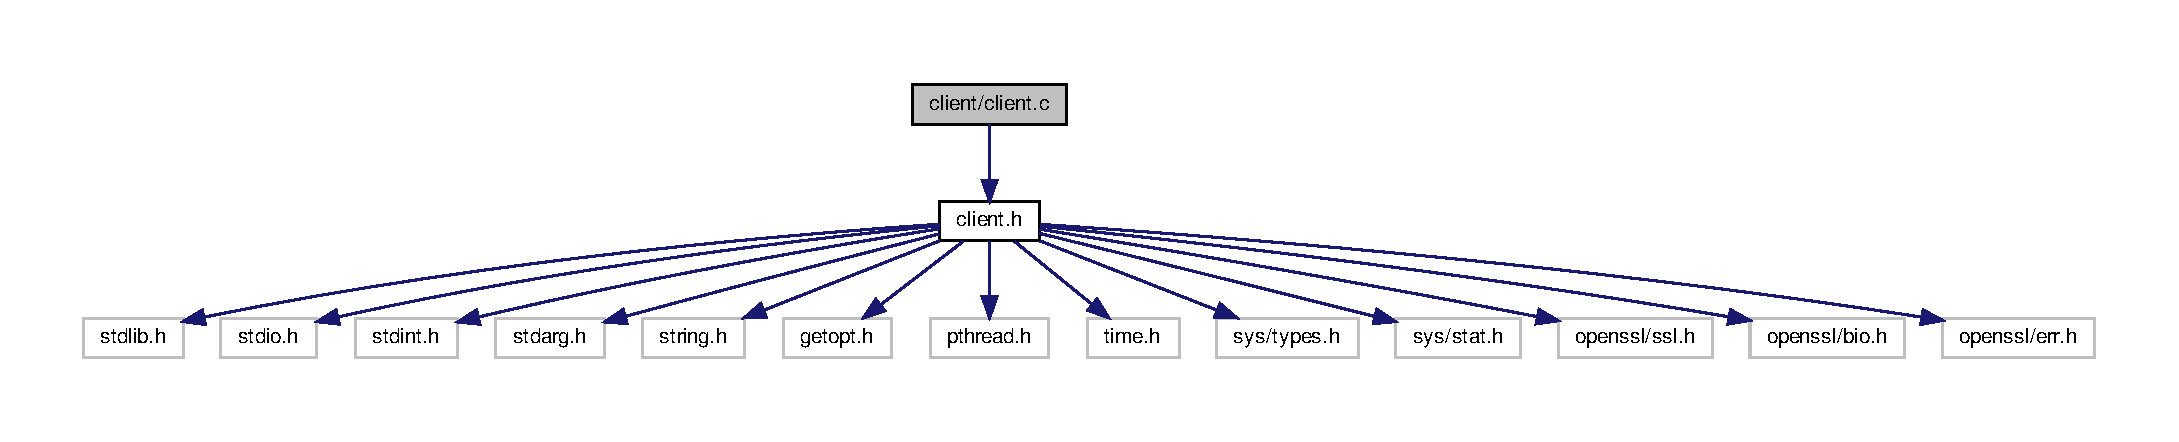
\includegraphics[width=350pt]{client_8c__incl}
\end{center}
\end{figure}
\subsection*{Functions}
\begin{DoxyCompactItemize}
\item 
\mbox{\Hypertarget{client_8c_a3c04138a5bfe5d72780bb7e82a18e627}\label{client_8c_a3c04138a5bfe5d72780bb7e82a18e627}} 
int {\bfseries main} (int argc, char $\ast$$\ast$argv)
\item 
B\+IO $\ast$ \hyperlink{client_8c_aa65d330efd2e64dbf42455681443ca34}{C\+L\+I\+E\+N\+T\+\_\+\+Attempt\+Connect} (S\+SL $\ast$ssl, S\+S\+L\+\_\+\+C\+TX $\ast$ctx, char $\ast$\hyperlink{client_8h_ab135e5154c1828bef226a3df98ee3333}{url})
\begin{DoxyCompactList}\small\item\em Attempt secure connection to the server specified by the url parameter. \end{DoxyCompactList}\item 
void $\ast$ \hyperlink{client_8c_a31fd8b95d88abb6d809a7320e4bd50fe}{C\+L\+I\+E\+N\+T\+\_\+\+Thread\+Handler} (void $\ast$args)
\begin{DoxyCompactList}\small\item\em Thread handler used for each client thread created. \end{DoxyCompactList}\item 
S\+S\+L\+\_\+\+C\+TX $\ast$ \hyperlink{client_8c_a3b5f000699c4f53e8615c1597b1c8f6e}{C\+L\+I\+E\+N\+T\+\_\+\+Init\+C\+TX} (void)
\begin{DoxyCompactList}\small\item\em Attempt to create an S\+SL context. \end{DoxyCompactList}\item 
uint8\+\_\+t \hyperlink{client_8c_a0306c39c0d5ad848227574db3a39dee3}{C\+L\+I\+E\+N\+T\+\_\+\+Write} (B\+IO $\ast$bio, char $\ast$buff)
\begin{DoxyCompactList}\small\item\em Attempts to write to the server. \end{DoxyCompactList}\item 
uint8\+\_\+t \hyperlink{client_8c_ae81077441665fb441e016d580b5a49b2}{C\+L\+I\+E\+N\+T\+\_\+\+Read} (B\+IO $\ast$bio, \hyperlink{client_8h_aba027bf73cecd0ccfad890748552be1c}{thread\+\_\+args} $\ast$thread\+Args)
\begin{DoxyCompactList}\small\item\em Attempts to read from the server. \end{DoxyCompactList}\end{DoxyCompactItemize}


\subsection{Detailed Description}
Client program able to establish an S\+SL connection to a specified server. 

\begin{DoxyAuthor}{Authors}
Douglas Healy (u16018100) 

Llewellyn Moyse (u15100708) 

Mohamed Ameen Omar (u16055323) 
\end{DoxyAuthor}
\begin{DoxyDate}{Date}
2019/02/14 
\end{DoxyDate}
\begin{DoxyVersion}{Version}
1.\+0 
\end{DoxyVersion}
\begin{DoxyCopyright}{Copyright}
Copyright \copyright{} 2019 -\/ E\+H\+N410 Group 7 
\end{DoxyCopyright}


\subsection{Function Documentation}
\mbox{\Hypertarget{client_8c_aa65d330efd2e64dbf42455681443ca34}\label{client_8c_aa65d330efd2e64dbf42455681443ca34}} 
\index{client.\+c@{client.\+c}!C\+L\+I\+E\+N\+T\+\_\+\+Attempt\+Connect@{C\+L\+I\+E\+N\+T\+\_\+\+Attempt\+Connect}}
\index{C\+L\+I\+E\+N\+T\+\_\+\+Attempt\+Connect@{C\+L\+I\+E\+N\+T\+\_\+\+Attempt\+Connect}!client.\+c@{client.\+c}}
\subsubsection{\texorpdfstring{C\+L\+I\+E\+N\+T\+\_\+\+Attempt\+Connect()}{CLIENT\_AttemptConnect()}}
{\footnotesize\ttfamily B\+IO$\ast$ C\+L\+I\+E\+N\+T\+\_\+\+Attempt\+Connect (\begin{DoxyParamCaption}\item[{S\+SL $\ast$}]{ssl,  }\item[{S\+S\+L\+\_\+\+C\+TX $\ast$}]{ctx,  }\item[{char $\ast$}]{url }\end{DoxyParamCaption})}



Attempt secure connection to the server specified by the url parameter. 


\begin{DoxyParams}{Parameters}
{\em ssl} & The S\+SL instance created by the client \\
\hline
{\em ctx} & The S\+SL context created by the client \\
\hline
{\em url} & The server location in the format \mbox{[}host\mbox{]}\+:\mbox{[}port\mbox{]} \\
\hline
\end{DoxyParams}
\begin{DoxyReturn}{Returns}
The B\+IO instance created if connection is successful 
\end{DoxyReturn}


Definition at line 134 of file client.\+c.

\mbox{\Hypertarget{client_8c_a3b5f000699c4f53e8615c1597b1c8f6e}\label{client_8c_a3b5f000699c4f53e8615c1597b1c8f6e}} 
\index{client.\+c@{client.\+c}!C\+L\+I\+E\+N\+T\+\_\+\+Init\+C\+TX@{C\+L\+I\+E\+N\+T\+\_\+\+Init\+C\+TX}}
\index{C\+L\+I\+E\+N\+T\+\_\+\+Init\+C\+TX@{C\+L\+I\+E\+N\+T\+\_\+\+Init\+C\+TX}!client.\+c@{client.\+c}}
\subsubsection{\texorpdfstring{C\+L\+I\+E\+N\+T\+\_\+\+Init\+C\+T\+X()}{CLIENT\_InitCTX()}}
{\footnotesize\ttfamily S\+S\+L\+\_\+\+C\+TX$\ast$ C\+L\+I\+E\+N\+T\+\_\+\+Init\+C\+TX (\begin{DoxyParamCaption}\item[{void}]{ }\end{DoxyParamCaption})}



Attempt to create an S\+SL context. 

\begin{DoxyReturn}{Returns}
The S\+SL context if instantiation was successful 
\end{DoxyReturn}


Definition at line 185 of file client.\+c.

Here is the caller graph for this function\+:\nopagebreak
\begin{figure}[H]
\begin{center}
\leavevmode
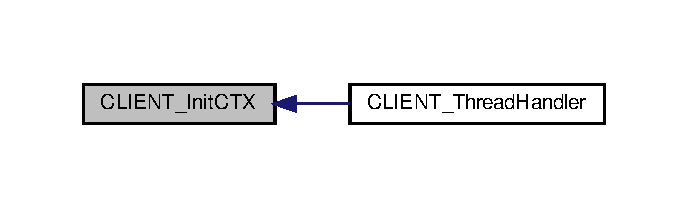
\includegraphics[width=330pt]{client_8c_a3b5f000699c4f53e8615c1597b1c8f6e_icgraph}
\end{center}
\end{figure}
\mbox{\Hypertarget{client_8c_ae81077441665fb441e016d580b5a49b2}\label{client_8c_ae81077441665fb441e016d580b5a49b2}} 
\index{client.\+c@{client.\+c}!C\+L\+I\+E\+N\+T\+\_\+\+Read@{C\+L\+I\+E\+N\+T\+\_\+\+Read}}
\index{C\+L\+I\+E\+N\+T\+\_\+\+Read@{C\+L\+I\+E\+N\+T\+\_\+\+Read}!client.\+c@{client.\+c}}
\subsubsection{\texorpdfstring{C\+L\+I\+E\+N\+T\+\_\+\+Read()}{CLIENT\_Read()}}
{\footnotesize\ttfamily uint8\+\_\+t C\+L\+I\+E\+N\+T\+\_\+\+Read (\begin{DoxyParamCaption}\item[{B\+IO $\ast$}]{bio,  }\item[{\hyperlink{client_8h_aba027bf73cecd0ccfad890748552be1c}{thread\+\_\+args} $\ast$}]{thread\+Args }\end{DoxyParamCaption})}



Attempts to read from the server. 


\begin{DoxyParams}{Parameters}
{\em bio} & The B\+IO instance created when establishing a connection to the server \\
\hline
{\em thread\+Args} & Encapsulated thread arguments containing the thread index and ID \\
\hline
\end{DoxyParams}
\begin{DoxyReturn}{Returns}
T\+R\+UE for a successful read / F\+A\+L\+SE for unsuccessful read 
\end{DoxyReturn}


Definition at line 207 of file client.\+c.

\mbox{\Hypertarget{client_8c_a31fd8b95d88abb6d809a7320e4bd50fe}\label{client_8c_a31fd8b95d88abb6d809a7320e4bd50fe}} 
\index{client.\+c@{client.\+c}!C\+L\+I\+E\+N\+T\+\_\+\+Thread\+Handler@{C\+L\+I\+E\+N\+T\+\_\+\+Thread\+Handler}}
\index{C\+L\+I\+E\+N\+T\+\_\+\+Thread\+Handler@{C\+L\+I\+E\+N\+T\+\_\+\+Thread\+Handler}!client.\+c@{client.\+c}}
\subsubsection{\texorpdfstring{C\+L\+I\+E\+N\+T\+\_\+\+Thread\+Handler()}{CLIENT\_ThreadHandler()}}
{\footnotesize\ttfamily void$\ast$ C\+L\+I\+E\+N\+T\+\_\+\+Thread\+Handler (\begin{DoxyParamCaption}\item[{void $\ast$}]{thread\+Args }\end{DoxyParamCaption})}



Thread handler used for each client thread created. 


\begin{DoxyParams}{Parameters}
{\em thread\+Args} & the encapsulated thread arguments containing the thread index and ID \\
\hline
\end{DoxyParams}
\begin{DoxyReturn}{Returns}

\end{DoxyReturn}


Definition at line 157 of file client.\+c.

Here is the call graph for this function\+:\nopagebreak
\begin{figure}[H]
\begin{center}
\leavevmode
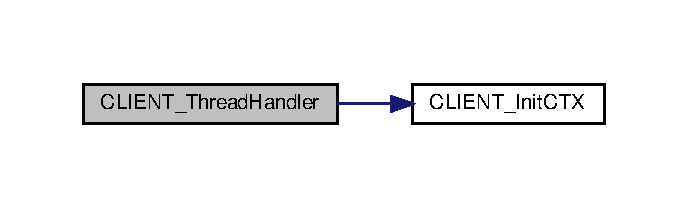
\includegraphics[width=330pt]{client_8c_a31fd8b95d88abb6d809a7320e4bd50fe_cgraph}
\end{center}
\end{figure}
\mbox{\Hypertarget{client_8c_a0306c39c0d5ad848227574db3a39dee3}\label{client_8c_a0306c39c0d5ad848227574db3a39dee3}} 
\index{client.\+c@{client.\+c}!C\+L\+I\+E\+N\+T\+\_\+\+Write@{C\+L\+I\+E\+N\+T\+\_\+\+Write}}
\index{C\+L\+I\+E\+N\+T\+\_\+\+Write@{C\+L\+I\+E\+N\+T\+\_\+\+Write}!client.\+c@{client.\+c}}
\subsubsection{\texorpdfstring{C\+L\+I\+E\+N\+T\+\_\+\+Write()}{CLIENT\_Write()}}
{\footnotesize\ttfamily uint8\+\_\+t C\+L\+I\+E\+N\+T\+\_\+\+Write (\begin{DoxyParamCaption}\item[{B\+IO $\ast$}]{bio,  }\item[{char $\ast$}]{buff }\end{DoxyParamCaption})}



Attempts to write to the server. 


\begin{DoxyParams}{Parameters}
{\em bio} & The B\+IO instance created when establishing a connection to the server \\
\hline
{\em buff} & Buffer to be written to the server \\
\hline
\end{DoxyParams}
\begin{DoxyReturn}{Returns}
T\+R\+UE for a successful write / F\+A\+L\+SE for an unsuccessful write 
\end{DoxyReturn}


Definition at line 196 of file client.\+c.


\hypertarget{client_8h}{}\section{client/client.h File Reference}
\label{client_8h}\index{client/client.\+h@{client/client.\+h}}


Client program able to establish an S\+SL connection to a specified server.  


{\ttfamily \#include $<$stdlib.\+h$>$}\newline
{\ttfamily \#include $<$stdio.\+h$>$}\newline
{\ttfamily \#include $<$stdint.\+h$>$}\newline
{\ttfamily \#include $<$stdarg.\+h$>$}\newline
{\ttfamily \#include $<$string.\+h$>$}\newline
{\ttfamily \#include $<$getopt.\+h$>$}\newline
{\ttfamily \#include $<$pthread.\+h$>$}\newline
{\ttfamily \#include $<$time.\+h$>$}\newline
{\ttfamily \#include $<$sys/types.\+h$>$}\newline
{\ttfamily \#include $<$sys/stat.\+h$>$}\newline
{\ttfamily \#include $<$openssl/ssl.\+h$>$}\newline
{\ttfamily \#include $<$openssl/bio.\+h$>$}\newline
{\ttfamily \#include $<$openssl/err.\+h$>$}\newline
Include dependency graph for client.\+h\+:\nopagebreak
\begin{figure}[H]
\begin{center}
\leavevmode
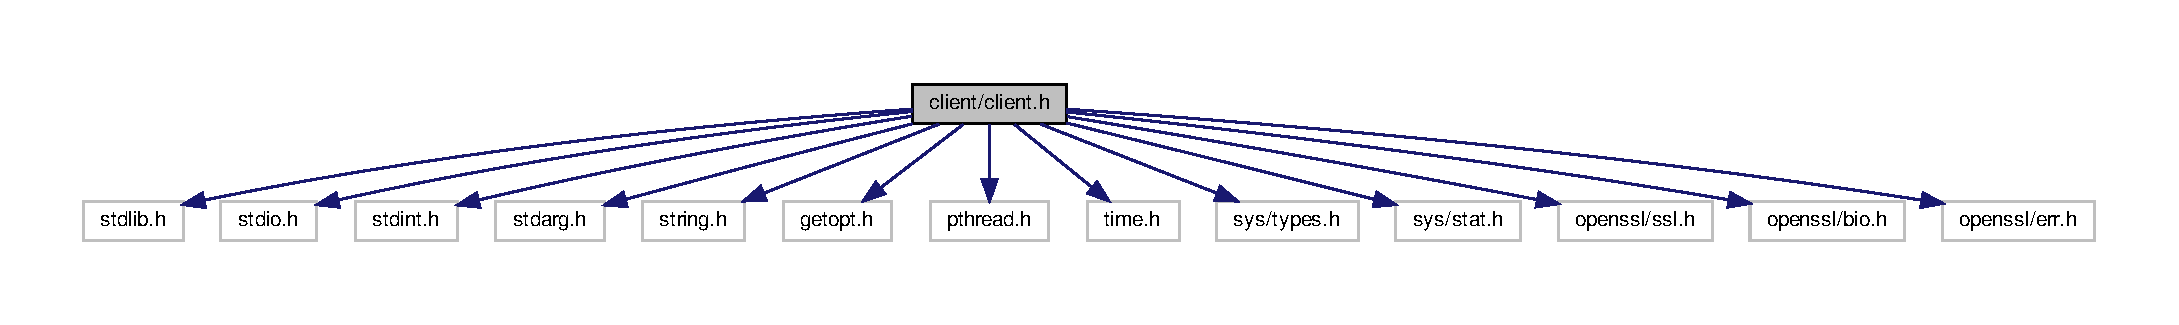
\includegraphics[width=350pt]{client_8h__incl}
\end{center}
\end{figure}
This graph shows which files directly or indirectly include this file\+:\nopagebreak
\begin{figure}[H]
\begin{center}
\leavevmode
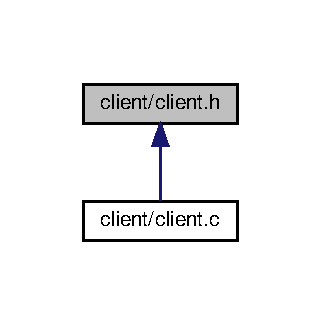
\includegraphics[width=154pt]{client_8h__dep__incl}
\end{center}
\end{figure}
\subsection*{Data Structures}
\begin{DoxyCompactItemize}
\item 
struct \hyperlink{struct__thread__args}{\+\_\+thread\+\_\+args}
\begin{DoxyCompactList}\small\item\em A structure used to encapsulate arguments sent to a new client thread handler. \end{DoxyCompactList}\end{DoxyCompactItemize}
\subsection*{Macros}
\begin{DoxyCompactItemize}
\item 
\mbox{\Hypertarget{client_8h_a45b6ee479d2daaf80ef51ad238c65c0d}\label{client_8h_a45b6ee479d2daaf80ef51ad238c65c0d}} 
\#define \hyperlink{client_8h_a45b6ee479d2daaf80ef51ad238c65c0d}{W\+R\+I\+T\+E\+\_\+\+B\+U\+F\+F\+E\+R\+\_\+\+S\+I\+ZE}~4096
\begin{DoxyCompactList}\small\item\em Buffer size used when writing to server. \end{DoxyCompactList}\item 
\mbox{\Hypertarget{client_8h_a46167a977503a51eb6efe97e870568c3}\label{client_8h_a46167a977503a51eb6efe97e870568c3}} 
\#define \hyperlink{client_8h_a46167a977503a51eb6efe97e870568c3}{R\+E\+A\+D\+\_\+\+B\+U\+F\+F\+E\+R\+\_\+\+S\+I\+ZE}~1024
\begin{DoxyCompactList}\small\item\em Buffer size used when reading from server. \end{DoxyCompactList}\item 
\mbox{\Hypertarget{client_8h_a8c8470adc3ccde16403efe9095394ed3}\label{client_8h_a8c8470adc3ccde16403efe9095394ed3}} 
\#define {\bfseries H\+T\+T\+P\+\_\+\+D\+E\+L\+IM}~\char`\"{}\textbackslash{}r\textbackslash{}n\char`\"{}
\item 
\mbox{\Hypertarget{client_8h_a2addad933336573674896d1a711e81ea}\label{client_8h_a2addad933336573674896d1a711e81ea}} 
\#define {\bfseries H\+T\+T\+P\+\_\+\+S\+P\+A\+CE}~\char`\"{} \char`\"{}
\item 
\mbox{\Hypertarget{client_8h_a061d2cb1ab385faaf63cf0a4f954ae8d}\label{client_8h_a061d2cb1ab385faaf63cf0a4f954ae8d}} 
\#define {\bfseries H\+T\+T\+P\+\_\+\+C\+O\+N\+T\+E\+N\+T\+\_\+\+T\+Y\+PE}~\char`\"{}Content-\/Type\+:\char`\"{}
\item 
\mbox{\Hypertarget{client_8h_aaf8ab78e79f73b4322567e511941284d}\label{client_8h_aaf8ab78e79f73b4322567e511941284d}} 
\#define {\bfseries H\+T\+T\+P\+\_\+\+C\+O\+N\+T\+E\+N\+T\+\_\+\+L\+E\+G\+N\+TH}~\char`\"{}Content-\/Length\+:\char`\"{}
\item 
\mbox{\Hypertarget{client_8h_a01b63621cc4ee9561aecfaf991e8f4c2}\label{client_8h_a01b63621cc4ee9561aecfaf991e8f4c2}} 
\#define \hyperlink{client_8h_a01b63621cc4ee9561aecfaf991e8f4c2}{H\+T\+T\+P\+\_\+\+D\+O\+W\+N\+L\+O\+A\+D\+\_\+\+P\+A\+TH}~\char`\"{}downloads\char`\"{}
\begin{DoxyCompactList}\small\item\em Download path where client will download the specified file to, this can be defined at compile time. \end{DoxyCompactList}\item 
\mbox{\Hypertarget{client_8h_a4fbfb8d38c4df01aa223ca1b6d593001}\label{client_8h_a4fbfb8d38c4df01aa223ca1b6d593001}} 
\#define {\bfseries C\+O\+L\+O\+U\+R\+\_\+\+R\+ED}~\char`\"{}\textbackslash{}x1B\mbox{[}31m\char`\"{}
\item 
\mbox{\Hypertarget{client_8h_aab830cc3243af7f74b77327aa26ab23f}\label{client_8h_aab830cc3243af7f74b77327aa26ab23f}} 
\#define {\bfseries C\+O\+L\+O\+U\+R\+\_\+\+G\+RN}~\char`\"{}\textbackslash{}x1B\mbox{[}32m\char`\"{}
\item 
\mbox{\Hypertarget{client_8h_a3c6a639021ff35a0fb905612a4edc557}\label{client_8h_a3c6a639021ff35a0fb905612a4edc557}} 
\#define {\bfseries C\+O\+L\+O\+U\+R\+\_\+\+Y\+EL}~\char`\"{}\textbackslash{}x1B\mbox{[}33m\char`\"{}
\item 
\mbox{\Hypertarget{client_8h_a58d9de6964db95bb879e64a755958377}\label{client_8h_a58d9de6964db95bb879e64a755958377}} 
\#define {\bfseries C\+O\+L\+O\+U\+R\+\_\+\+B\+LU}~\char`\"{}\textbackslash{}x1B\mbox{[}34m\char`\"{}
\item 
\mbox{\Hypertarget{client_8h_aa8ff9cf949a91e20b865ed7d998dd4c5}\label{client_8h_aa8ff9cf949a91e20b865ed7d998dd4c5}} 
\#define {\bfseries C\+O\+L\+O\+U\+R\+\_\+\+M\+AG}~\char`\"{}\textbackslash{}x1B\mbox{[}35m\char`\"{}
\item 
\mbox{\Hypertarget{client_8h_a487172a29c4c42e481856dd9882d83b1}\label{client_8h_a487172a29c4c42e481856dd9882d83b1}} 
\#define {\bfseries C\+O\+L\+O\+U\+R\+\_\+\+C\+YN}~\char`\"{}\textbackslash{}x1B\mbox{[}36m\char`\"{}
\item 
\mbox{\Hypertarget{client_8h_a147267dcde16a76bdc81cde399e41d06}\label{client_8h_a147267dcde16a76bdc81cde399e41d06}} 
\#define {\bfseries C\+O\+L\+O\+U\+R\+\_\+\+W\+HT}~\char`\"{}\textbackslash{}x1B\mbox{[}37m\char`\"{}
\item 
\mbox{\Hypertarget{client_8h_aba77d52b0fce6e966578f939d1e2a42d}\label{client_8h_aba77d52b0fce6e966578f939d1e2a42d}} 
\#define {\bfseries C\+O\+L\+O\+U\+R\+\_\+\+R\+E\+S\+ET}~\char`\"{}\textbackslash{}x1B\mbox{[}0m\char`\"{}
\item 
\mbox{\Hypertarget{client_8h_aa8cecfc5c5c054d2875c03e77b7be15d}\label{client_8h_aa8cecfc5c5c054d2875c03e77b7be15d}} 
\#define {\bfseries T\+R\+UE}~(1 == 1)
\item 
\mbox{\Hypertarget{client_8h_aa93f0eb578d23995850d61f7d61c55c1}\label{client_8h_aa93f0eb578d23995850d61f7d61c55c1}} 
\#define {\bfseries F\+A\+L\+SE}~(1 == 0)
\item 
\mbox{\Hypertarget{client_8h_ad6497a312321c3e7e38848affdd00032}\label{client_8h_ad6497a312321c3e7e38848affdd00032}} 
\#define {\bfseries trace}(f\+\_\+,  args...)
\item 
\mbox{\Hypertarget{client_8h_ac7bf88f07107bb69d3817c857a4117c4}\label{client_8h_ac7bf88f07107bb69d3817c857a4117c4}} 
\#define {\bfseries \+\_\+printf}(f\+\_\+,  args...)~printf(f\+\_\+\char`\"{}\textbackslash{}r\textbackslash{}n\char`\"{}, \#\#args)
\end{DoxyCompactItemize}
\subsection*{Typedefs}
\begin{DoxyCompactItemize}
\item 
\mbox{\Hypertarget{client_8h_aba027bf73cecd0ccfad890748552be1c}\label{client_8h_aba027bf73cecd0ccfad890748552be1c}} 
typedef struct \hyperlink{struct__thread__args}{\+\_\+thread\+\_\+args} \hyperlink{client_8h_aba027bf73cecd0ccfad890748552be1c}{thread\+\_\+args}
\begin{DoxyCompactList}\small\item\em A structure used to encapsulate arguments sent to a new client thread handler. \end{DoxyCompactList}\end{DoxyCompactItemize}
\subsection*{Functions}
\begin{DoxyCompactItemize}
\item 
void $\ast$ \hyperlink{client_8h_a3df7ecac9e73a53b8278020a216cff88}{C\+L\+I\+E\+N\+T\+\_\+\+Thread\+Handler} (void $\ast$thread\+Args)
\begin{DoxyCompactList}\small\item\em Thread handler used for each client thread created. \end{DoxyCompactList}\item 
B\+IO $\ast$ \hyperlink{client_8h_aa65d330efd2e64dbf42455681443ca34}{C\+L\+I\+E\+N\+T\+\_\+\+Attempt\+Connect} (S\+SL $\ast$ssl, S\+S\+L\+\_\+\+C\+TX $\ast$ctx, char $\ast$\hyperlink{client_8h_ab135e5154c1828bef226a3df98ee3333}{url})
\begin{DoxyCompactList}\small\item\em Attempt secure connection to the server specified by the url parameter. \end{DoxyCompactList}\item 
S\+S\+L\+\_\+\+C\+TX $\ast$ \hyperlink{client_8h_a3b5f000699c4f53e8615c1597b1c8f6e}{C\+L\+I\+E\+N\+T\+\_\+\+Init\+C\+TX} (void)
\begin{DoxyCompactList}\small\item\em Attempt to create an S\+SL context. \end{DoxyCompactList}\item 
uint8\+\_\+t \hyperlink{client_8h_a0306c39c0d5ad848227574db3a39dee3}{C\+L\+I\+E\+N\+T\+\_\+\+Write} (B\+IO $\ast$bio, char $\ast$buff)
\begin{DoxyCompactList}\small\item\em Attempts to write to the server. \end{DoxyCompactList}\item 
uint8\+\_\+t \hyperlink{client_8h_ae81077441665fb441e016d580b5a49b2}{C\+L\+I\+E\+N\+T\+\_\+\+Read} (B\+IO $\ast$bio, \hyperlink{client_8h_aba027bf73cecd0ccfad890748552be1c}{thread\+\_\+args} $\ast$thread\+Args)
\begin{DoxyCompactList}\small\item\em Attempts to read from the server. \end{DoxyCompactList}\end{DoxyCompactItemize}
\subsection*{Variables}
\begin{DoxyCompactItemize}
\item 
\mbox{\Hypertarget{client_8h_ae813f75c9e72b199987413ff955e54d8}\label{client_8h_ae813f75c9e72b199987413ff955e54d8}} 
B\+IO $\ast$ \hyperlink{client_8h_ae813f75c9e72b199987413ff955e54d8}{outbio} = N\+U\+LL
\begin{DoxyCompactList}\small\item\em B\+IO instance used for printing errors. \end{DoxyCompactList}\item 
\mbox{\Hypertarget{client_8h_ab135e5154c1828bef226a3df98ee3333}\label{client_8h_ab135e5154c1828bef226a3df98ee3333}} 
char $\ast$ \hyperlink{client_8h_ab135e5154c1828bef226a3df98ee3333}{url} = N\+U\+LL
\begin{DoxyCompactList}\small\item\em The url of the server in the format \mbox{[}host\mbox{]}\+:\mbox{[}port\mbox{]}. \end{DoxyCompactList}\item 
\mbox{\Hypertarget{client_8h_a44196e6a5696d10442c29e639437196e}\label{client_8h_a44196e6a5696d10442c29e639437196e}} 
char $\ast$ \hyperlink{client_8h_a44196e6a5696d10442c29e639437196e}{path} = N\+U\+LL
\begin{DoxyCompactList}\small\item\em The path to the file to be downloaded, must contain file extension. \end{DoxyCompactList}\item 
\mbox{\Hypertarget{client_8h_ab79a8e6eceff978df17adfefd24c157a}\label{client_8h_ab79a8e6eceff978df17adfefd24c157a}} 
char $\ast$ \hyperlink{client_8h_ab79a8e6eceff978df17adfefd24c157a}{file\+Ext}
\begin{DoxyCompactList}\small\item\em The file name of the file to download which is obtained from the given path. \end{DoxyCompactList}\item 
\mbox{\Hypertarget{client_8h_a1dffaa86d425273d26de380b7fcef769}\label{client_8h_a1dffaa86d425273d26de380b7fcef769}} 
uint32\+\_\+t \hyperlink{client_8h_a1dffaa86d425273d26de380b7fcef769}{client\+Instances} = 1
\begin{DoxyCompactList}\small\item\em Number of client instances which is defined by -\/n command-\/line argument, defaults to 1. \end{DoxyCompactList}\end{DoxyCompactItemize}


\subsection{Detailed Description}
Client program able to establish an S\+SL connection to a specified server. 

\begin{DoxyAuthor}{Authors}
Douglas Healy (u16018100) 

Llewellyn Moyse (u15100708) 

Mohamed Ameen Omar (u16055323) 
\end{DoxyAuthor}
\begin{DoxyDate}{Date}
2019/02/14 
\end{DoxyDate}
\begin{DoxyVersion}{Version}
1.\+0 
\end{DoxyVersion}
\begin{DoxyCopyright}{Copyright}
Copyright \copyright{} 2019 -\/ E\+H\+N410 Group 7 
\end{DoxyCopyright}


\subsection{Function Documentation}
\mbox{\Hypertarget{client_8h_aa65d330efd2e64dbf42455681443ca34}\label{client_8h_aa65d330efd2e64dbf42455681443ca34}} 
\index{client.\+h@{client.\+h}!C\+L\+I\+E\+N\+T\+\_\+\+Attempt\+Connect@{C\+L\+I\+E\+N\+T\+\_\+\+Attempt\+Connect}}
\index{C\+L\+I\+E\+N\+T\+\_\+\+Attempt\+Connect@{C\+L\+I\+E\+N\+T\+\_\+\+Attempt\+Connect}!client.\+h@{client.\+h}}
\subsubsection{\texorpdfstring{C\+L\+I\+E\+N\+T\+\_\+\+Attempt\+Connect()}{CLIENT\_AttemptConnect()}}
{\footnotesize\ttfamily B\+IO$\ast$ C\+L\+I\+E\+N\+T\+\_\+\+Attempt\+Connect (\begin{DoxyParamCaption}\item[{S\+SL $\ast$}]{ssl,  }\item[{S\+S\+L\+\_\+\+C\+TX $\ast$}]{ctx,  }\item[{char $\ast$}]{url }\end{DoxyParamCaption})}



Attempt secure connection to the server specified by the url parameter. 


\begin{DoxyParams}{Parameters}
{\em ssl} & The S\+SL instance created by the client \\
\hline
{\em ctx} & The S\+SL context created by the client \\
\hline
{\em url} & The server location in the format \mbox{[}host\mbox{]}\+:\mbox{[}port\mbox{]} \\
\hline
\end{DoxyParams}
\begin{DoxyReturn}{Returns}
The B\+IO instance created if connection is successful 
\end{DoxyReturn}


Definition at line 134 of file client.\+c.

\mbox{\Hypertarget{client_8h_a3b5f000699c4f53e8615c1597b1c8f6e}\label{client_8h_a3b5f000699c4f53e8615c1597b1c8f6e}} 
\index{client.\+h@{client.\+h}!C\+L\+I\+E\+N\+T\+\_\+\+Init\+C\+TX@{C\+L\+I\+E\+N\+T\+\_\+\+Init\+C\+TX}}
\index{C\+L\+I\+E\+N\+T\+\_\+\+Init\+C\+TX@{C\+L\+I\+E\+N\+T\+\_\+\+Init\+C\+TX}!client.\+h@{client.\+h}}
\subsubsection{\texorpdfstring{C\+L\+I\+E\+N\+T\+\_\+\+Init\+C\+T\+X()}{CLIENT\_InitCTX()}}
{\footnotesize\ttfamily S\+S\+L\+\_\+\+C\+TX$\ast$ C\+L\+I\+E\+N\+T\+\_\+\+Init\+C\+TX (\begin{DoxyParamCaption}\item[{void}]{ }\end{DoxyParamCaption})}



Attempt to create an S\+SL context. 

\begin{DoxyReturn}{Returns}
The S\+SL context if instantiation was successful 
\end{DoxyReturn}


Definition at line 185 of file client.\+c.

Here is the caller graph for this function\+:\nopagebreak
\begin{figure}[H]
\begin{center}
\leavevmode
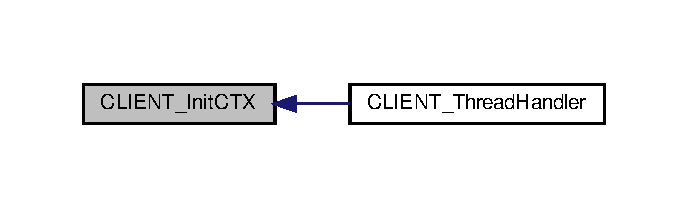
\includegraphics[width=330pt]{client_8h_a3b5f000699c4f53e8615c1597b1c8f6e_icgraph}
\end{center}
\end{figure}
\mbox{\Hypertarget{client_8h_ae81077441665fb441e016d580b5a49b2}\label{client_8h_ae81077441665fb441e016d580b5a49b2}} 
\index{client.\+h@{client.\+h}!C\+L\+I\+E\+N\+T\+\_\+\+Read@{C\+L\+I\+E\+N\+T\+\_\+\+Read}}
\index{C\+L\+I\+E\+N\+T\+\_\+\+Read@{C\+L\+I\+E\+N\+T\+\_\+\+Read}!client.\+h@{client.\+h}}
\subsubsection{\texorpdfstring{C\+L\+I\+E\+N\+T\+\_\+\+Read()}{CLIENT\_Read()}}
{\footnotesize\ttfamily uint8\+\_\+t C\+L\+I\+E\+N\+T\+\_\+\+Read (\begin{DoxyParamCaption}\item[{B\+IO $\ast$}]{bio,  }\item[{\hyperlink{client_8h_aba027bf73cecd0ccfad890748552be1c}{thread\+\_\+args} $\ast$}]{thread\+Args }\end{DoxyParamCaption})}



Attempts to read from the server. 


\begin{DoxyParams}{Parameters}
{\em bio} & The B\+IO instance created when establishing a connection to the server \\
\hline
{\em thread\+Args} & Encapsulated thread arguments containing the thread index and ID \\
\hline
\end{DoxyParams}
\begin{DoxyReturn}{Returns}
T\+R\+UE for a successful read / F\+A\+L\+SE for unsuccessful read 
\end{DoxyReturn}


Definition at line 207 of file client.\+c.

\mbox{\Hypertarget{client_8h_a3df7ecac9e73a53b8278020a216cff88}\label{client_8h_a3df7ecac9e73a53b8278020a216cff88}} 
\index{client.\+h@{client.\+h}!C\+L\+I\+E\+N\+T\+\_\+\+Thread\+Handler@{C\+L\+I\+E\+N\+T\+\_\+\+Thread\+Handler}}
\index{C\+L\+I\+E\+N\+T\+\_\+\+Thread\+Handler@{C\+L\+I\+E\+N\+T\+\_\+\+Thread\+Handler}!client.\+h@{client.\+h}}
\subsubsection{\texorpdfstring{C\+L\+I\+E\+N\+T\+\_\+\+Thread\+Handler()}{CLIENT\_ThreadHandler()}}
{\footnotesize\ttfamily void$\ast$ C\+L\+I\+E\+N\+T\+\_\+\+Thread\+Handler (\begin{DoxyParamCaption}\item[{void $\ast$}]{thread\+Args }\end{DoxyParamCaption})}



Thread handler used for each client thread created. 


\begin{DoxyParams}{Parameters}
{\em thread\+Args} & the encapsulated thread arguments containing the thread index and ID \\
\hline
\end{DoxyParams}
\begin{DoxyReturn}{Returns}

\end{DoxyReturn}


Definition at line 157 of file client.\+c.

Here is the call graph for this function\+:\nopagebreak
\begin{figure}[H]
\begin{center}
\leavevmode
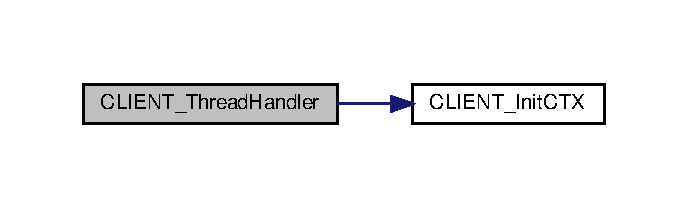
\includegraphics[width=330pt]{client_8h_a3df7ecac9e73a53b8278020a216cff88_cgraph}
\end{center}
\end{figure}
\mbox{\Hypertarget{client_8h_a0306c39c0d5ad848227574db3a39dee3}\label{client_8h_a0306c39c0d5ad848227574db3a39dee3}} 
\index{client.\+h@{client.\+h}!C\+L\+I\+E\+N\+T\+\_\+\+Write@{C\+L\+I\+E\+N\+T\+\_\+\+Write}}
\index{C\+L\+I\+E\+N\+T\+\_\+\+Write@{C\+L\+I\+E\+N\+T\+\_\+\+Write}!client.\+h@{client.\+h}}
\subsubsection{\texorpdfstring{C\+L\+I\+E\+N\+T\+\_\+\+Write()}{CLIENT\_Write()}}
{\footnotesize\ttfamily uint8\+\_\+t C\+L\+I\+E\+N\+T\+\_\+\+Write (\begin{DoxyParamCaption}\item[{B\+IO $\ast$}]{bio,  }\item[{char $\ast$}]{buff }\end{DoxyParamCaption})}



Attempts to write to the server. 


\begin{DoxyParams}{Parameters}
{\em bio} & The B\+IO instance created when establishing a connection to the server \\
\hline
{\em buff} & Buffer to be written to the server \\
\hline
\end{DoxyParams}
\begin{DoxyReturn}{Returns}
T\+R\+UE for a successful write / F\+A\+L\+SE for an unsuccessful write 
\end{DoxyReturn}


Definition at line 196 of file client.\+c.


\hypertarget{server_8c}{}\section{server/server.c File Reference}
\label{server_8c}\index{server/server.\+c@{server/server.\+c}}


Server function implementation file. This file contains the function implementation source code used to run the ssl server.  


{\ttfamily \#include \char`\"{}server.\+h\char`\"{}}\newline
Include dependency graph for server.\+c\+:\nopagebreak
\begin{figure}[H]
\begin{center}
\leavevmode
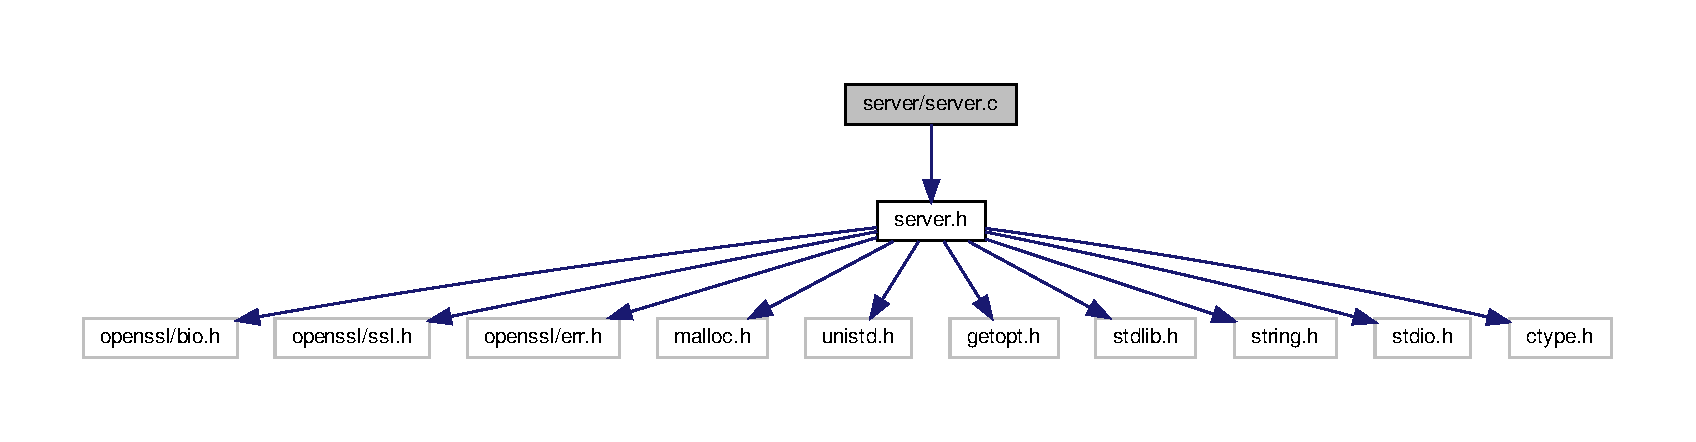
\includegraphics[width=350pt]{server_8c__incl}
\end{center}
\end{figure}
\subsection*{Functions}
\begin{DoxyCompactItemize}
\item 
\mbox{\Hypertarget{server_8c_a0d20b69b0ad703df78459e1033d5c1d4}\label{server_8c_a0d20b69b0ad703df78459e1033d5c1d4}} 
void \hyperlink{server_8c_a0d20b69b0ad703df78459e1033d5c1d4}{print\+Help} ()
\begin{DoxyCompactList}\small\item\em Function name\+: print\+Help Prints out the help menu or usage menu for the ssl server. Called when the user inputs invalid parameters or the -\/h (help) flag is set by the user. \end{DoxyCompactList}\item 
char $\ast$ \hyperlink{server_8c_a01985a8e0c7ec3719ebe2dba272a02d8}{find\+Port} (int counter)
\begin{DoxyCompactList}\small\item\em Function name\+: find\+Port Used as a helper function to find a open port for the server to bind to. This function uses the port 4000 as a base port and adds the contents of. \end{DoxyCompactList}\item 
void $\ast$ \hyperlink{server_8c_a5800d02353519f21ac22f5dbfbee2ace}{the\+Server} (void $\ast$bio\+Ptr)
\begin{DoxyCompactList}\small\item\em Function name\+: the\+Server. Intended use is as a multithreaded function. Used to thread the server listening on a port. Should the server not be able to bind the specifed port, it will spawn a new thread to the \hyperlink{server_8c_a180f1d916084d821a9e99136064ab071}{smart\+Server()} function in order to find a reasonable open port and this function will end. Should the server have the ability to bind to the specified port, it will bind to it and run and inifinite loop listening for socket connections on that port. Once a client attempts to make a connection, the function will spawn a new thread for that client -\/ running the \hyperlink{server_8c_a9fc618a14fcb2dd88c05a0e6aa63fdc5}{a\+Client()} function allowing for multiple clients to be handled simultaneously, each within its own thread. \end{DoxyCompactList}\item 
void $\ast$ \hyperlink{server_8c_a9fc618a14fcb2dd88c05a0e6aa63fdc5}{a\+Client} (void $\ast$socket)
\begin{DoxyCompactList}\small\item\em Function name\+: a\+Client This a function intended to be used in a multithreaded manner. This function handles a connection between the secure ssl server and the client. \end{DoxyCompactList}\item 
char $\ast$ \hyperlink{server_8c_abbda488be5be6184f753da54e577d6e2}{parse\+Request} (char $\ast$temp)
\begin{DoxyCompactList}\small\item\em Function name\+: parse\+Request This function processing the request received from the client. Since the ssl server only supports \char`\"{}\+G\+E\+T\char`\"{} http requests, it scans the request received given in. \end{DoxyCompactList}\item 
void \hyperlink{server_8c_ae6e604b8d08d6060dcb643b9b923862c}{send\+Response} (B\+IO $\ast$socket, char $\ast$resource)
\begin{DoxyCompactList}\small\item\em Function name\+: send\+Response This function is used to send the requested file given by. \end{DoxyCompactList}\item 
char $\ast$ \hyperlink{server_8c_a72ca4593d1fb624fd2a6ae8c7d9ab68c}{construct\+Header} (char $\ast$status\+Code, unsigned long length, char $\ast$mime\+Type)
\begin{DoxyCompactList}\small\item\em Function name\+: construct\+Header This function constrcuts the response header sent to a client from the ssl server. Based off of the. \end{DoxyCompactList}\item 
void \hyperlink{server_8c_a21455a45359c92447df5cc064ee2ae58}{send\+File} (B\+IO $\ast$socket, char $\ast$file\+Name, char $\ast$status\+Code)
\begin{DoxyCompactList}\small\item\em Function name\+: send\+File This function sends or writes the appripate file to the B\+IO object/socket connected to the client. The function attempts to open the file with the path given by. \end{DoxyCompactList}\item 
void $\ast$ \hyperlink{server_8c_a180f1d916084d821a9e99136064ab071}{smart\+Server} ()
\begin{DoxyCompactList}\small\item\em Function name\+: smart\+Server. This function is a multithreaded function called when the requested port or default port for the S\+SL server could not be binded to, due to the port being blocked, restricted or already reserved. \end{DoxyCompactList}\item 
char $\ast$ \hyperlink{server_8c_a7751c5c6e765ed5ce531c15904682eab}{get\+Mime\+Type} (char $\ast$name)
\begin{DoxyCompactList}\small\item\em T\+Function name\+: get\+Mime\+Type This function is used to determine the mime-\/type of the file passed in as a paramter. It extracts the file extension of the filename passed in as. \end{DoxyCompactList}\end{DoxyCompactItemize}
\subsection*{Variables}
\begin{DoxyCompactItemize}
\item 
\mbox{\Hypertarget{server_8c_acf5cd4c5a9ada37a9bd90a80be3e21dd}\label{server_8c_acf5cd4c5a9ada37a9bd90a80be3e21dd}} 
char \hyperlink{server_8c_acf5cd4c5a9ada37a9bd90a80be3e21dd}{connected\+Port} \mbox{[}S\+T\+R\+I\+N\+G\+\_\+\+S\+I\+ZE\mbox{]} = \char`\"{}empty\char`\"{}
\begin{DoxyCompactList}\small\item\em used to output the current port on which the server is listening. \end{DoxyCompactList}\item 
\mbox{\Hypertarget{server_8c_acb96fb4e0856037c018d840c905c1375}\label{server_8c_acb96fb4e0856037c018d840c905c1375}} 
char \hyperlink{server_8c_acb96fb4e0856037c018d840c905c1375}{connected\+Host} \mbox{[}S\+T\+R\+I\+N\+G\+\_\+\+S\+I\+ZE\mbox{]} = \char`\"{}empty\char`\"{}
\begin{DoxyCompactList}\small\item\em used to output the current hostname on which the server is listening. \end{DoxyCompactList}\end{DoxyCompactItemize}


\subsection{Detailed Description}
Server function implementation file. This file contains the function implementation source code used to run the ssl server. 

\begin{DoxyAuthor}{Authors}
Mohamed Ameen Omar (u16055323) 

Douglas Healy (u16018100) 

Llewellyn Moyse (u15100708) 
\end{DoxyAuthor}
\begin{DoxyVersion}{Version}
0.\+1 
\end{DoxyVersion}
\begin{DoxyDate}{Date}
2019-\/02-\/13
\end{DoxyDate}
\begin{DoxyCopyright}{Copyright}
Copyright \copyright{} 2019 -\/ E\+HN 410 Group 7 
\end{DoxyCopyright}


\subsection{Function Documentation}
\mbox{\Hypertarget{server_8c_a9fc618a14fcb2dd88c05a0e6aa63fdc5}\label{server_8c_a9fc618a14fcb2dd88c05a0e6aa63fdc5}} 
\index{server.\+c@{server.\+c}!a\+Client@{a\+Client}}
\index{a\+Client@{a\+Client}!server.\+c@{server.\+c}}
\subsubsection{\texorpdfstring{a\+Client()}{aClient()}}
{\footnotesize\ttfamily void$\ast$ a\+Client (\begin{DoxyParamCaption}\item[{void $\ast$}]{socket }\end{DoxyParamCaption})}



Function name\+: a\+Client This a function intended to be used in a multithreaded manner. This function handles a connection between the secure ssl server and the client. 

This function is spawned when a client connects to the server. The function first performs the ssl handhake to ensure that the connection between the server and the client is secure. If the handshake fails for whatever reason, the connection is terminated and the function returns. Thereafter the client request is read into a buffer. If the client request could not be read or the connection has been disconnected, the function terminates the connection (if connected) and returns. Once the client request is successfully read, the request is processed and the response is sent or written to the requested client. Thereafter the connection to the client is terminated and the function returns.

This function is called in a new thread each time a new client request is received, since each new request is a new connection. The server does not store any information about a client after the connection is terminated and each connection is treated as the first initial connection.


\begin{DoxyParams}{Parameters}
{\em socket} & -\/ B\+I\+O$\ast$ pointing to a bio object that is connected to the client. The socket on which the current connection is done. \\
\hline
\end{DoxyParams}
\begin{DoxyReturn}{Returns}
void$\ast$ -\/ Returns N\+U\+LL, since the intended use is as a P\+O\+S\+IX compliant threaded function 
\end{DoxyReturn}


Definition at line 121 of file server.\+c.

Here is the call graph for this function\+:\nopagebreak
\begin{figure}[H]
\begin{center}
\leavevmode
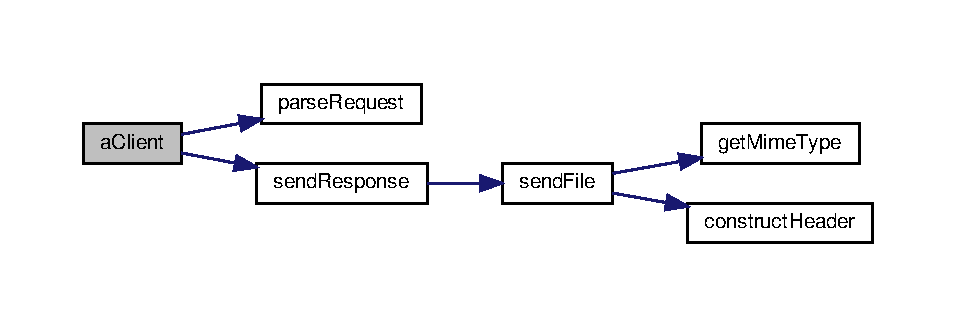
\includegraphics[width=350pt]{server_8c_a9fc618a14fcb2dd88c05a0e6aa63fdc5_cgraph}
\end{center}
\end{figure}
Here is the caller graph for this function\+:\nopagebreak
\begin{figure}[H]
\begin{center}
\leavevmode
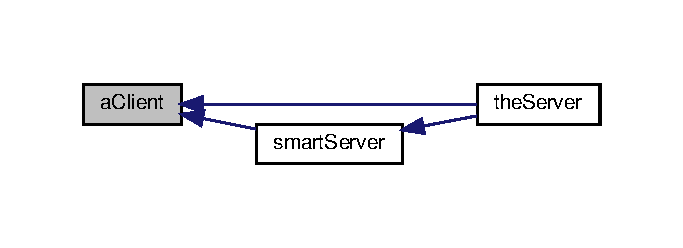
\includegraphics[width=328pt]{server_8c_a9fc618a14fcb2dd88c05a0e6aa63fdc5_icgraph}
\end{center}
\end{figure}
\mbox{\Hypertarget{server_8c_a72ca4593d1fb624fd2a6ae8c7d9ab68c}\label{server_8c_a72ca4593d1fb624fd2a6ae8c7d9ab68c}} 
\index{server.\+c@{server.\+c}!construct\+Header@{construct\+Header}}
\index{construct\+Header@{construct\+Header}!server.\+c@{server.\+c}}
\subsubsection{\texorpdfstring{construct\+Header()}{constructHeader()}}
{\footnotesize\ttfamily char$\ast$ construct\+Header (\begin{DoxyParamCaption}\item[{char $\ast$}]{status\+Code,  }\item[{unsigned long}]{length,  }\item[{char $\ast$}]{mime\+Type }\end{DoxyParamCaption})}



Function name\+: construct\+Header This function constrcuts the response header sent to a client from the ssl server. Based off of the. 


\begin{DoxyParams}{Parameters}
{\em status\+Code} & it constructs the appropiate response, the length of the response as well as the mime\+Type of the response file sent back to the client. Constructs the header according to the H\+T\+TP version 1.\+1 standard.\\
\hline
\end{DoxyParams}
returns the response header to be sent to the client.


\begin{DoxyParams}{Parameters}
{\em status\+Code} & -\/ char$\ast$ to a C-\/\+String object containing the response status code to be sent to the client. \\
\hline
{\em length} & -\/ unsigned long containing the length in bytes of the amount of data to be sent to client \\
\hline
{\em mime\+Type} & -\/ char$\ast$ to a C-\/\+String object contsaing the apprtiate mime-\/type of the data to be sent as a response to the client request. \\
\hline
\end{DoxyParams}
\begin{DoxyReturn}{Returns}
char$\ast$ -\/ the constructed response header. 
\end{DoxyReturn}


Definition at line 283 of file server.\+c.

Here is the caller graph for this function\+:\nopagebreak
\begin{figure}[H]
\begin{center}
\leavevmode
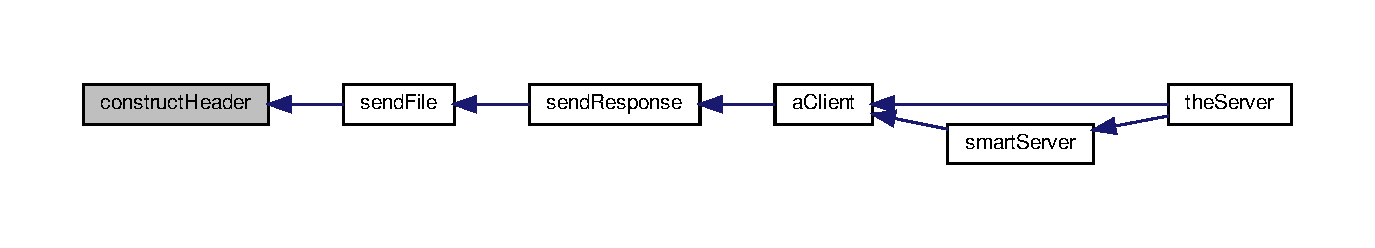
\includegraphics[width=350pt]{server_8c_a72ca4593d1fb624fd2a6ae8c7d9ab68c_icgraph}
\end{center}
\end{figure}
\mbox{\Hypertarget{server_8c_a01985a8e0c7ec3719ebe2dba272a02d8}\label{server_8c_a01985a8e0c7ec3719ebe2dba272a02d8}} 
\index{server.\+c@{server.\+c}!find\+Port@{find\+Port}}
\index{find\+Port@{find\+Port}!server.\+c@{server.\+c}}
\subsubsection{\texorpdfstring{find\+Port()}{findPort()}}
{\footnotesize\ttfamily char$\ast$ find\+Port (\begin{DoxyParamCaption}\item[{int}]{counter }\end{DoxyParamCaption})}



Function name\+: find\+Port Used as a helper function to find a open port for the server to bind to. This function uses the port 4000 as a base port and adds the contents of. 


\begin{DoxyParams}{Parameters}
{\em counter} & to 4000. Returns the string representation of the proposed port. Note\+: Does not check whether the \char`\"{}counter\char`\"{} variable is beyond a certain threshold -\/ implementation specific. Does error checking to determine if the contents of \\
\hline
{\em counter} & is an integer. If it is not \char`\"{}-\/1\char`\"{} is returned to signify a problem.\\
\hline
{\em counter} & -\/ Type\+: Integer. Contents of which are added to 4000 to specify a proposed port. \\
\hline
\end{DoxyParams}
\begin{DoxyReturn}{Returns}
char$\ast$ -\/ The string representation of the proposed port. 
\end{DoxyReturn}


Definition at line 49 of file server.\+c.

Here is the caller graph for this function\+:\nopagebreak
\begin{figure}[H]
\begin{center}
\leavevmode
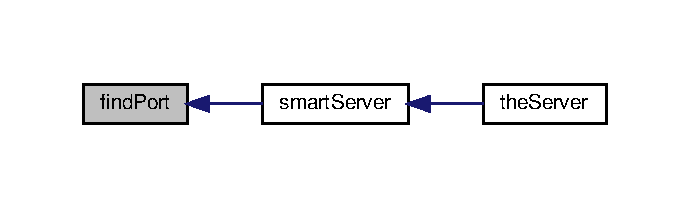
\includegraphics[width=331pt]{server_8c_a01985a8e0c7ec3719ebe2dba272a02d8_icgraph}
\end{center}
\end{figure}
\mbox{\Hypertarget{server_8c_a7751c5c6e765ed5ce531c15904682eab}\label{server_8c_a7751c5c6e765ed5ce531c15904682eab}} 
\index{server.\+c@{server.\+c}!get\+Mime\+Type@{get\+Mime\+Type}}
\index{get\+Mime\+Type@{get\+Mime\+Type}!server.\+c@{server.\+c}}
\subsubsection{\texorpdfstring{get\+Mime\+Type()}{getMimeType()}}
{\footnotesize\ttfamily char$\ast$ get\+Mime\+Type (\begin{DoxyParamCaption}\item[{char $\ast$}]{name }\end{DoxyParamCaption})}



T\+Function name\+: get\+Mime\+Type This function is used to determine the mime-\/type of the file passed in as a paramter. It extracts the file extension of the filename passed in as. 


\begin{DoxyParams}{Parameters}
{\em name} & and searches the mime-\/types.\+tsv file for the appropriate mime-\/type.\\
\hline
\end{DoxyParams}
If the appropriate mime-\/type is found, it is returned as a char$\ast$, if not, the application/octet-\/stream mime-\/type is returned to indicate to the client that the mime-\/type for the file is unknown.

If a user wishes to add a mime-\/type + file extension combination to improve compatiblity, they may do so by editing the mime-\/types.\+tsv file found in the root directory of the server. Ensure that the format is adhered to and the number found on the first line of the file is incremented to ensure that the newly added mime-\/type is considered.


\begin{DoxyParams}{Parameters}
{\em name} & -\/ char$\ast$ pointing to a C-\/\+Style string containing the path to file to be sent to client. \\
\hline
\end{DoxyParams}
\begin{DoxyReturn}{Returns}
char$\ast$ -\/ the mime-\/type to use for the file requested. 
\end{DoxyReturn}


Definition at line 455 of file server.\+c.

Here is the caller graph for this function\+:\nopagebreak
\begin{figure}[H]
\begin{center}
\leavevmode
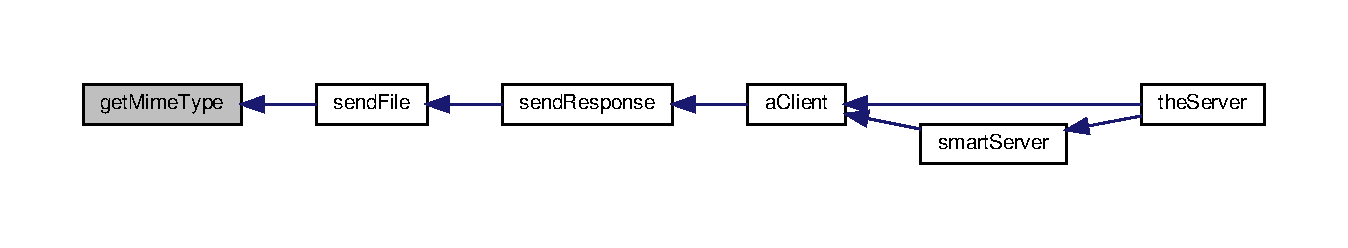
\includegraphics[width=350pt]{server_8c_a7751c5c6e765ed5ce531c15904682eab_icgraph}
\end{center}
\end{figure}
\mbox{\Hypertarget{server_8c_abbda488be5be6184f753da54e577d6e2}\label{server_8c_abbda488be5be6184f753da54e577d6e2}} 
\index{server.\+c@{server.\+c}!parse\+Request@{parse\+Request}}
\index{parse\+Request@{parse\+Request}!server.\+c@{server.\+c}}
\subsubsection{\texorpdfstring{parse\+Request()}{parseRequest()}}
{\footnotesize\ttfamily char$\ast$ parse\+Request (\begin{DoxyParamCaption}\item[{char $\ast$}]{temp }\end{DoxyParamCaption})}



Function name\+: parse\+Request This function processing the request received from the client. Since the ssl server only supports \char`\"{}\+G\+E\+T\char`\"{} http requests, it scans the request received given in. 


\begin{DoxyParams}{Parameters}
{\em temp,for} & the directory of the file requested.\\
\hline
\end{DoxyParams}
The requested file is then returned. If a requested file could not be found in the request header, due to H\+T\+TP protcol version mismatches or any other unknown reason, N\+U\+LL is returned.


\begin{DoxyParams}{Parameters}
{\em temp} & -\/ char$\ast$ poinuting to a C-\/\+String containing the request received from the client. \\
\hline
\end{DoxyParams}
\begin{DoxyReturn}{Returns}
char$\ast$ -\/ the requested file from the request header. N\+U\+LL if a file path could not be found in the request header. 
\end{DoxyReturn}


Definition at line 185 of file server.\+c.

Here is the caller graph for this function\+:\nopagebreak
\begin{figure}[H]
\begin{center}
\leavevmode
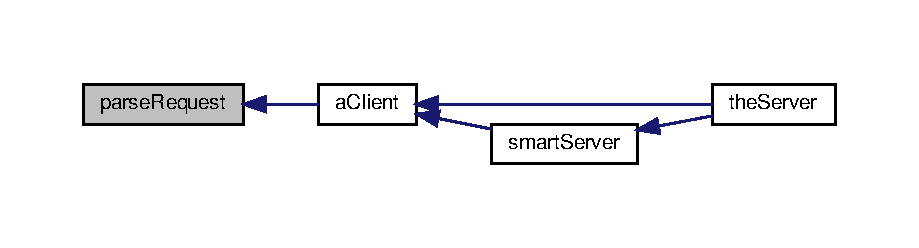
\includegraphics[width=350pt]{server_8c_abbda488be5be6184f753da54e577d6e2_icgraph}
\end{center}
\end{figure}
\mbox{\Hypertarget{server_8c_a21455a45359c92447df5cc064ee2ae58}\label{server_8c_a21455a45359c92447df5cc064ee2ae58}} 
\index{server.\+c@{server.\+c}!send\+File@{send\+File}}
\index{send\+File@{send\+File}!server.\+c@{server.\+c}}
\subsubsection{\texorpdfstring{send\+File()}{sendFile()}}
{\footnotesize\ttfamily void send\+File (\begin{DoxyParamCaption}\item[{B\+IO $\ast$}]{socket,  }\item[{char $\ast$}]{file\+Name,  }\item[{char $\ast$}]{status\+Code }\end{DoxyParamCaption})}



Function name\+: send\+File This function sends or writes the appripate file to the B\+IO object/socket connected to the client. The function attempts to open the file with the path given by. 


\begin{DoxyParams}{Parameters}
{\em file\+Name} & and writes the file in \char`\"{}chunks\char`\"{} of 2048 bytes. The contents of the opened file is read into a buffer and the contents of the buffer are written to the socket until the end of the file has been reached. The file is read at a rate of 2048 bytes per write. Once the entire contents of the file has been written the B\+IO object is flushed to ensure all data is sent and the function returns.\\
\hline
\end{DoxyParams}
This function first constructs the appropriate response header, sends the response header, thereafter sending or writing the requested file.

If the file could not be opened, due to it not existing in the root directory or sub-\/directory of the ssl server program, the function returns without writing anything to the client.


\begin{DoxyParams}{Parameters}
{\em socket} & -\/ B\+I\+O$\ast$ to a B\+IO object connecting the client to the ssl server. \\
\hline
{\em file\+Name} & -\/ char$\ast$ pointing to a C-\/\+String containing the requested file \\
\hline
{\em status\+Code} & -\/ char$\ast$ pointing to a C-\/\+String containing the appropiate status code to send to the client within the response header. \\
\hline
\end{DoxyParams}


Definition at line 328 of file server.\+c.

Here is the call graph for this function\+:\nopagebreak
\begin{figure}[H]
\begin{center}
\leavevmode
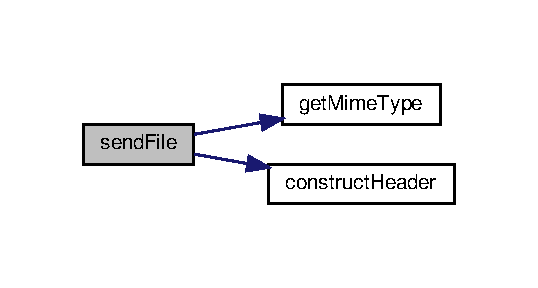
\includegraphics[width=258pt]{server_8c_a21455a45359c92447df5cc064ee2ae58_cgraph}
\end{center}
\end{figure}
Here is the caller graph for this function\+:\nopagebreak
\begin{figure}[H]
\begin{center}
\leavevmode
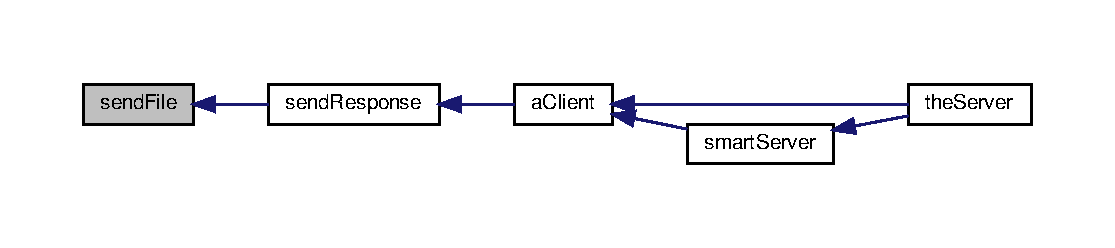
\includegraphics[width=350pt]{server_8c_a21455a45359c92447df5cc064ee2ae58_icgraph}
\end{center}
\end{figure}
\mbox{\Hypertarget{server_8c_ae6e604b8d08d6060dcb643b9b923862c}\label{server_8c_ae6e604b8d08d6060dcb643b9b923862c}} 
\index{server.\+c@{server.\+c}!send\+Response@{send\+Response}}
\index{send\+Response@{send\+Response}!server.\+c@{server.\+c}}
\subsubsection{\texorpdfstring{send\+Response()}{sendResponse()}}
{\footnotesize\ttfamily void send\+Response (\begin{DoxyParamCaption}\item[{B\+IO $\ast$}]{socket,  }\item[{char $\ast$}]{resource }\end{DoxyParamCaption})}



Function name\+: send\+Response This function is used to send the requested file given by. 


\begin{DoxyParams}{Parameters}
{\em resource} & to the client connected on \\
\hline
{\em socket.} & If the resoure is N\+U\+LL signalling that the request header was malformed, the page not found error html page is sent as a response to the client.\\
\hline
\end{DoxyParams}
If the ressource requested points to a directory or the requested file is not found, the page not found error page is sent as a response to the client.

If client sends a G\+ET / request to the server, the default index.\+html homepage is sent as a response.

If the requested resource could be found the server root directrory or sub directroy, it is sent to the client. The main purpose of this function is to determine which response is sent to the clinet. It calls the send\+File function to send/write the appropriate file to the B\+IO socket.


\begin{DoxyParams}{Parameters}
{\em socket} & -\/ B\+I\+O$\ast$ pointing to the B\+IO object on which the client is paired/connected. \\
\hline
{\em resource} & -\/ char$\ast$ pointing to a c-\/string object conting the path to the requested resoure received from the clinet. N\+U\+LL if the client sent a malformed request. \\
\hline
\end{DoxyParams}


Definition at line 228 of file server.\+c.

Here is the call graph for this function\+:\nopagebreak
\begin{figure}[H]
\begin{center}
\leavevmode
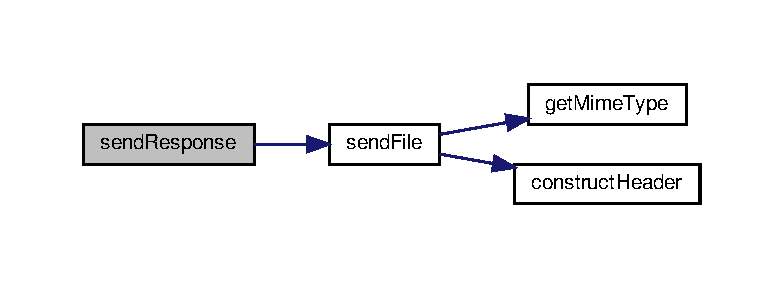
\includegraphics[width=350pt]{server_8c_ae6e604b8d08d6060dcb643b9b923862c_cgraph}
\end{center}
\end{figure}
Here is the caller graph for this function\+:\nopagebreak
\begin{figure}[H]
\begin{center}
\leavevmode
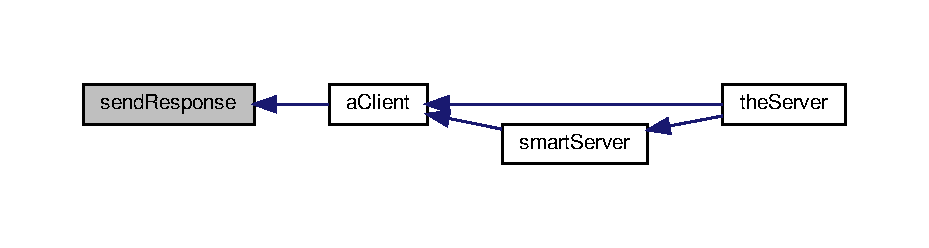
\includegraphics[width=350pt]{server_8c_ae6e604b8d08d6060dcb643b9b923862c_icgraph}
\end{center}
\end{figure}
\mbox{\Hypertarget{server_8c_a180f1d916084d821a9e99136064ab071}\label{server_8c_a180f1d916084d821a9e99136064ab071}} 
\index{server.\+c@{server.\+c}!smart\+Server@{smart\+Server}}
\index{smart\+Server@{smart\+Server}!server.\+c@{server.\+c}}
\subsubsection{\texorpdfstring{smart\+Server()}{smartServer()}}
{\footnotesize\ttfamily void$\ast$ smart\+Server (\begin{DoxyParamCaption}{ }\end{DoxyParamCaption})}



Function name\+: smart\+Server. This function is a multithreaded function called when the requested port or default port for the S\+SL server could not be binded to, due to the port being blocked, restricted or already reserved. 

This function attempts to bind to an alternate port within the range 4000-\/4049. If no port within this range could be binded to the function ends the program, alerts; the user that no port could be found and requests the user re-\/run the ssl server with an alternate port speciifed.

If a port could be binded to it functions in the same manner as the function the\+Server. See function\+: the\+Server.

\begin{DoxyReturn}{Returns}
void$\ast$ -\/ N\+U\+LL to signify the end of the thread. 
\end{DoxyReturn}


Definition at line 378 of file server.\+c.

Here is the call graph for this function\+:\nopagebreak
\begin{figure}[H]
\begin{center}
\leavevmode
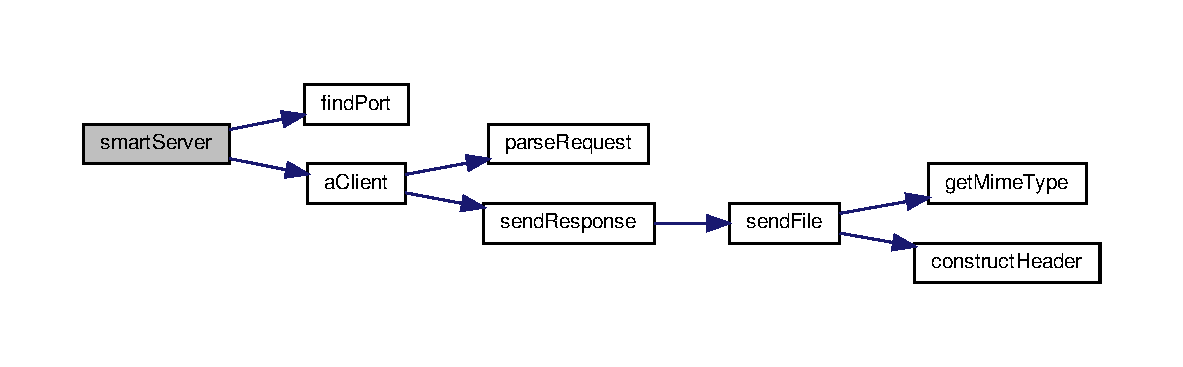
\includegraphics[width=350pt]{server_8c_a180f1d916084d821a9e99136064ab071_cgraph}
\end{center}
\end{figure}
Here is the caller graph for this function\+:\nopagebreak
\begin{figure}[H]
\begin{center}
\leavevmode
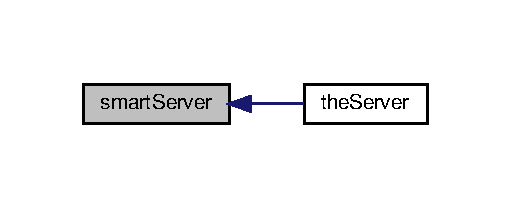
\includegraphics[width=245pt]{server_8c_a180f1d916084d821a9e99136064ab071_icgraph}
\end{center}
\end{figure}
\mbox{\Hypertarget{server_8c_a5800d02353519f21ac22f5dbfbee2ace}\label{server_8c_a5800d02353519f21ac22f5dbfbee2ace}} 
\index{server.\+c@{server.\+c}!the\+Server@{the\+Server}}
\index{the\+Server@{the\+Server}!server.\+c@{server.\+c}}
\subsubsection{\texorpdfstring{the\+Server()}{theServer()}}
{\footnotesize\ttfamily void$\ast$ the\+Server (\begin{DoxyParamCaption}\item[{void $\ast$}]{bio\+Ptr }\end{DoxyParamCaption})}



Function name\+: the\+Server. Intended use is as a multithreaded function. Used to thread the server listening on a port. Should the server not be able to bind the specifed port, it will spawn a new thread to the \hyperlink{server_8c_a180f1d916084d821a9e99136064ab071}{smart\+Server()} function in order to find a reasonable open port and this function will end. Should the server have the ability to bind to the specified port, it will bind to it and run and inifinite loop listening for socket connections on that port. Once a client attempts to make a connection, the function will spawn a new thread for that client -\/ running the \hyperlink{server_8c_a9fc618a14fcb2dd88c05a0e6aa63fdc5}{a\+Client()} function allowing for multiple clients to be handled simultaneously, each within its own thread. 


\begin{DoxyParams}{Parameters}
{\em bio\+Ptr} & -\/ B\+I\+O$\ast$ pointing to a B\+IO object with the ssl and tcp wrapping already implemented to enable a listening socket \\
\hline
\end{DoxyParams}
\begin{DoxyReturn}{Returns}
void$\ast$ -\/ Returns N\+U\+LL, since the intended use is as a P\+O\+S\+IX threaded function 
\end{DoxyReturn}


Definition at line 68 of file server.\+c.

Here is the call graph for this function\+:\nopagebreak
\begin{figure}[H]
\begin{center}
\leavevmode
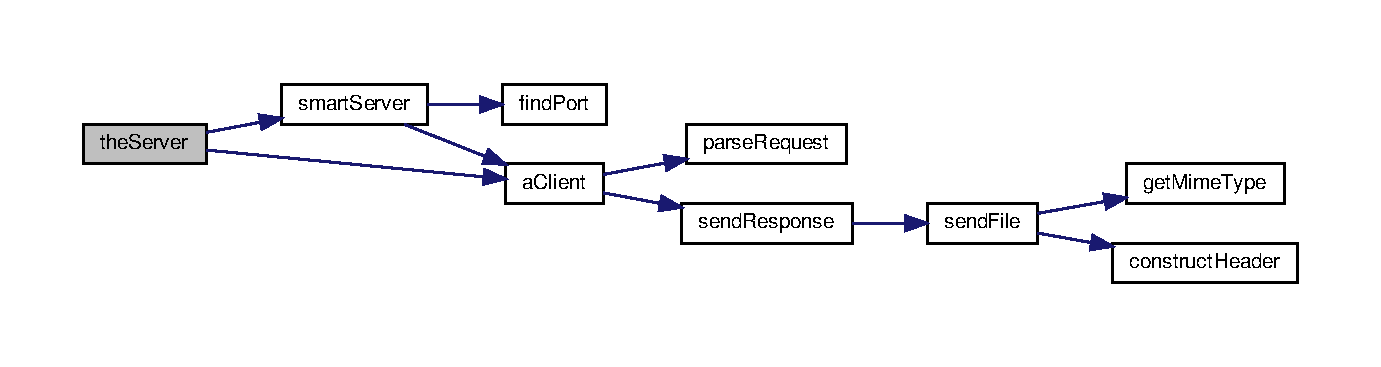
\includegraphics[width=350pt]{server_8c_a5800d02353519f21ac22f5dbfbee2ace_cgraph}
\end{center}
\end{figure}

\hypertarget{server_8h}{}\section{server/server.h File Reference}
\label{server_8h}\index{server/server.\+h@{server/server.\+h}}


Header This header provides the function protypes and constants used in the implementation of the B\+IO S\+SL threaded server. See files \hyperlink{server_main_8c}{server\+Main.\+c} and \hyperlink{server_8c}{server.\+c}.  


{\ttfamily \#include \char`\"{}openssl/bio.\+h\char`\"{}}\newline
{\ttfamily \#include \char`\"{}openssl/ssl.\+h\char`\"{}}\newline
{\ttfamily \#include \char`\"{}openssl/err.\+h\char`\"{}}\newline
{\ttfamily \#include \char`\"{}malloc.\+h\char`\"{}}\newline
{\ttfamily \#include \char`\"{}unistd.\+h\char`\"{}}\newline
{\ttfamily \#include \char`\"{}getopt.\+h\char`\"{}}\newline
{\ttfamily \#include $<$stdlib.\+h$>$}\newline
{\ttfamily \#include $<$string.\+h$>$}\newline
{\ttfamily \#include $<$stdio.\+h$>$}\newline
{\ttfamily \#include $<$ctype.\+h$>$}\newline
Include dependency graph for server.\+h\+:\nopagebreak
\begin{figure}[H]
\begin{center}
\leavevmode
\includegraphics[width=350pt]{server_8h__incl}
\end{center}
\end{figure}
This graph shows which files directly or indirectly include this file\+:\nopagebreak
\begin{figure}[H]
\begin{center}
\leavevmode
\includegraphics[width=284pt]{server_8h__dep__incl}
\end{center}
\end{figure}
\subsection*{Macros}
\begin{DoxyCompactItemize}
\item 
\mbox{\Hypertarget{server_8h_ad78224efe1d3fb39b67ca74ad9d9eec7}\label{server_8h_ad78224efe1d3fb39b67ca74ad9d9eec7}} 
\#define {\bfseries S\+T\+R\+I\+N\+G\+\_\+\+S\+I\+ZE}~80
\item 
\mbox{\Hypertarget{server_8h_a581612b7b0d68a0fe79f39038687b86c}\label{server_8h_a581612b7b0d68a0fe79f39038687b86c}} 
\#define {\bfseries M\+I\+M\+E\+T\+Y\+PE}~\char`\"{}mime-\/types.\+tsv\char`\"{}
\end{DoxyCompactItemize}
\subsection*{Functions}
\begin{DoxyCompactItemize}
\item 
char $\ast$ \hyperlink{server_8h_a2cdb41d0910c3a1d4b82668182dd8a33}{find\+Port} (int)
\begin{DoxyCompactList}\small\item\em Function name\+: find\+Port Used as a helper function to find a open port for the server to bind to. This function uses the port 4000 as a base port and adds the contents of. \end{DoxyCompactList}\item 
char $\ast$ \hyperlink{server_8h_a7751c5c6e765ed5ce531c15904682eab}{get\+Mime\+Type} (char $\ast$name)
\begin{DoxyCompactList}\small\item\em T\+Function name\+: get\+Mime\+Type This function is used to determine the mime-\/type of the file passed in as a paramter. It extracts the file extension of the filename passed in as. \end{DoxyCompactList}\item 
char $\ast$ \hyperlink{server_8h_a74ba0703eb52435c76e95d5976205593}{construct\+Header} (char $\ast$, unsigned long, char $\ast$)
\begin{DoxyCompactList}\small\item\em Function name\+: construct\+Header This function constrcuts the response header sent to a client from the ssl server. Based off of the. \end{DoxyCompactList}\item 
char $\ast$ \hyperlink{server_8h_ada7020aa14056fa9a6c85f8181ca3d09}{parse\+Request} (char $\ast$)
\begin{DoxyCompactList}\small\item\em Function name\+: parse\+Request This function processing the request received from the client. Since the ssl server only supports \char`\"{}\+G\+E\+T\char`\"{} http requests, it scans the request received given in. \end{DoxyCompactList}\item 
void \hyperlink{server_8h_a9162818fd6dab1ab1d6ea625b9fd6b12}{send\+Response} (B\+IO $\ast$, char $\ast$)
\begin{DoxyCompactList}\small\item\em Function name\+: send\+Response This function is used to send the requested file given by. \end{DoxyCompactList}\item 
\mbox{\Hypertarget{server_8h_a0d20b69b0ad703df78459e1033d5c1d4}\label{server_8h_a0d20b69b0ad703df78459e1033d5c1d4}} 
void \hyperlink{server_8h_a0d20b69b0ad703df78459e1033d5c1d4}{print\+Help} ()
\begin{DoxyCompactList}\small\item\em Function name\+: print\+Help Prints out the help menu or usage menu for the ssl server. Called when the user inputs invalid parameters or the -\/h (help) flag is set by the user. \end{DoxyCompactList}\item 
void $\ast$ \hyperlink{server_8h_a12f20281e4906f4d25c7c059993ddbc1}{the\+Server} (void $\ast$)
\begin{DoxyCompactList}\small\item\em Function name\+: the\+Server. Intended use is as a multithreaded function. Used to thread the server listening on a port. Should the server not be able to bind the specifed port, it will spawn a new thread to the \hyperlink{server_8h_a180f1d916084d821a9e99136064ab071}{smart\+Server()} function in order to find a reasonable open port and this function will end. Should the server have the ability to bind to the specified port, it will bind to it and run and inifinite loop listening for socket connections on that port. Once a client attempts to make a connection, the function will spawn a new thread for that client -\/ running the \hyperlink{server_8h_af7fd23153c3e547bf7dcde194ffce209}{a\+Client()} function allowing for multiple clients to be handled simultaneously, each within its own thread. \end{DoxyCompactList}\item 
void \hyperlink{server_8h_a02ad7b3294dd3cdda69bb9295aaaf7ed}{send\+File} (B\+IO $\ast$socket, char $\ast$, char $\ast$)
\begin{DoxyCompactList}\small\item\em Function name\+: send\+File This function sends or writes the appripate file to the B\+IO object/socket connected to the client. The function attempts to open the file with the path given by. \end{DoxyCompactList}\item 
void $\ast$ \hyperlink{server_8h_af7fd23153c3e547bf7dcde194ffce209}{a\+Client} (void $\ast$)
\begin{DoxyCompactList}\small\item\em Function name\+: a\+Client This a function intended to be used in a multithreaded manner. This function handles a connection between the secure ssl server and the client. \end{DoxyCompactList}\item 
void $\ast$ \hyperlink{server_8h_a180f1d916084d821a9e99136064ab071}{smart\+Server} ()
\begin{DoxyCompactList}\small\item\em Function name\+: smart\+Server. This function is a multithreaded function called when the requested port or default port for the S\+SL server could not be binded to, due to the port being blocked, restricted or already reserved. \end{DoxyCompactList}\end{DoxyCompactItemize}
\subsection*{Variables}
\begin{DoxyCompactItemize}
\item 
\mbox{\Hypertarget{server_8h_acf5cd4c5a9ada37a9bd90a80be3e21dd}\label{server_8h_acf5cd4c5a9ada37a9bd90a80be3e21dd}} 
char \hyperlink{server_8h_acf5cd4c5a9ada37a9bd90a80be3e21dd}{connected\+Port} \mbox{[}S\+T\+R\+I\+N\+G\+\_\+\+S\+I\+ZE\mbox{]}
\begin{DoxyCompactList}\small\item\em used to output the current port on which the server is listening. \end{DoxyCompactList}\item 
\mbox{\Hypertarget{server_8h_acb96fb4e0856037c018d840c905c1375}\label{server_8h_acb96fb4e0856037c018d840c905c1375}} 
char \hyperlink{server_8h_acb96fb4e0856037c018d840c905c1375}{connected\+Host} \mbox{[}S\+T\+R\+I\+N\+G\+\_\+\+S\+I\+ZE\mbox{]}
\begin{DoxyCompactList}\small\item\em used to output the current hostname on which the server is listening. \end{DoxyCompactList}\end{DoxyCompactItemize}


\subsection{Detailed Description}
Header This header provides the function protypes and constants used in the implementation of the B\+IO S\+SL threaded server. See files \hyperlink{server_main_8c}{server\+Main.\+c} and \hyperlink{server_8c}{server.\+c}. 

\begin{DoxyAuthor}{Authors}
Mohamed Ameen Omar (u16055323) 

Douglas Healy (u16018100) 

Llewellyn Moyse (u15100708) 
\end{DoxyAuthor}
\begin{DoxyCopyright}{Copyright}
Copyright \copyright{} 2019 -\/ E\+HN 410 Group 7 
\end{DoxyCopyright}


\subsection{Function Documentation}
\mbox{\Hypertarget{server_8h_af7fd23153c3e547bf7dcde194ffce209}\label{server_8h_af7fd23153c3e547bf7dcde194ffce209}} 
\index{server.\+h@{server.\+h}!a\+Client@{a\+Client}}
\index{a\+Client@{a\+Client}!server.\+h@{server.\+h}}
\subsubsection{\texorpdfstring{a\+Client()}{aClient()}}
{\footnotesize\ttfamily void$\ast$ a\+Client (\begin{DoxyParamCaption}\item[{void $\ast$}]{socket }\end{DoxyParamCaption})}



Function name\+: a\+Client This a function intended to be used in a multithreaded manner. This function handles a connection between the secure ssl server and the client. 

This function is spawned when a client connects to the server. The function first performs the ssl handhake to ensure that the connection between the server and the client is secure. If the handshake fails for whatever reason, the connection is terminated and the function returns. Thereafter the client request is read into a buffer. If the client request could not be read or the connection has been disconnected, the function terminates the connection (if connected) and returns. Once the client request is successfully read, the request is processed and the response is sent or written to the requested client. Thereafter the connection to the client is terminated and the function returns.

This function is called in a new thread each time a new client request is received, since each new request is a new connection. The server does not store any information about a client after the connection is terminated and each connection is treated as the first initial connection.


\begin{DoxyParams}{Parameters}
{\em socket} & -\/ B\+I\+O$\ast$ pointing to a bio object that is connected to the client. The socket on which the current connection is done. \\
\hline
\end{DoxyParams}
\begin{DoxyReturn}{Returns}
void$\ast$ -\/ Returns N\+U\+LL, since the intended use is as a P\+O\+S\+IX compliant threaded function 
\end{DoxyReturn}


Definition at line 121 of file server.\+c.

Here is the call graph for this function\+:\nopagebreak
\begin{figure}[H]
\begin{center}
\leavevmode
\includegraphics[width=350pt]{server_8h_af7fd23153c3e547bf7dcde194ffce209_cgraph}
\end{center}
\end{figure}
Here is the caller graph for this function\+:\nopagebreak
\begin{figure}[H]
\begin{center}
\leavevmode
\includegraphics[width=328pt]{server_8h_af7fd23153c3e547bf7dcde194ffce209_icgraph}
\end{center}
\end{figure}
\mbox{\Hypertarget{server_8h_a74ba0703eb52435c76e95d5976205593}\label{server_8h_a74ba0703eb52435c76e95d5976205593}} 
\index{server.\+h@{server.\+h}!construct\+Header@{construct\+Header}}
\index{construct\+Header@{construct\+Header}!server.\+h@{server.\+h}}
\subsubsection{\texorpdfstring{construct\+Header()}{constructHeader()}}
{\footnotesize\ttfamily char$\ast$ construct\+Header (\begin{DoxyParamCaption}\item[{char $\ast$}]{status\+Code,  }\item[{unsigned long}]{length,  }\item[{char $\ast$}]{mime\+Type }\end{DoxyParamCaption})}



Function name\+: construct\+Header This function constrcuts the response header sent to a client from the ssl server. Based off of the. 


\begin{DoxyParams}{Parameters}
{\em status\+Code} & it constructs the appropiate response, the length of the response as well as the mime\+Type of the response file sent back to the client. Constructs the header according to the H\+T\+TP version 1.\+1 standard.\\
\hline
\end{DoxyParams}
returns the response header to be sent to the client.


\begin{DoxyParams}{Parameters}
{\em status\+Code} & -\/ char$\ast$ to a C-\/\+String object containing the response status code to be sent to the client. \\
\hline
{\em length} & -\/ unsigned long containing the length in bytes of the amount of data to be sent to client \\
\hline
{\em mime\+Type} & -\/ char$\ast$ to a C-\/\+String object contsaing the apprtiate mime-\/type of the data to be sent as a response to the client request. \\
\hline
\end{DoxyParams}
\begin{DoxyReturn}{Returns}
char$\ast$ -\/ the constructed response header. 
\end{DoxyReturn}


Definition at line 283 of file server.\+c.

Here is the caller graph for this function\+:\nopagebreak
\begin{figure}[H]
\begin{center}
\leavevmode
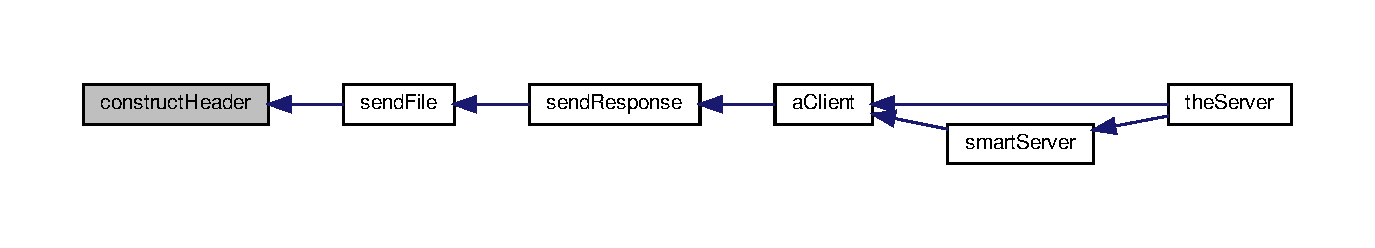
\includegraphics[width=350pt]{server_8h_a74ba0703eb52435c76e95d5976205593_icgraph}
\end{center}
\end{figure}
\mbox{\Hypertarget{server_8h_a2cdb41d0910c3a1d4b82668182dd8a33}\label{server_8h_a2cdb41d0910c3a1d4b82668182dd8a33}} 
\index{server.\+h@{server.\+h}!find\+Port@{find\+Port}}
\index{find\+Port@{find\+Port}!server.\+h@{server.\+h}}
\subsubsection{\texorpdfstring{find\+Port()}{findPort()}}
{\footnotesize\ttfamily char$\ast$ find\+Port (\begin{DoxyParamCaption}\item[{int}]{counter }\end{DoxyParamCaption})}



Function name\+: find\+Port Used as a helper function to find a open port for the server to bind to. This function uses the port 4000 as a base port and adds the contents of. 


\begin{DoxyParams}{Parameters}
{\em counter} & to 4000. Returns the string representation of the proposed port. Note\+: Does not check whether the \char`\"{}counter\char`\"{} variable is beyond a certain threshold -\/ implementation specific. Does error checking to determine if the contents of \\
\hline
{\em counter} & is an integer. If it is not \char`\"{}-\/1\char`\"{} is returned to signify a problem.\\
\hline
{\em counter} & -\/ Type\+: Integer. Contents of which are added to 4000 to specify a proposed port. \\
\hline
\end{DoxyParams}
\begin{DoxyReturn}{Returns}
char$\ast$ -\/ The string representation of the proposed port. 
\end{DoxyReturn}


Definition at line 49 of file server.\+c.

Here is the caller graph for this function\+:\nopagebreak
\begin{figure}[H]
\begin{center}
\leavevmode
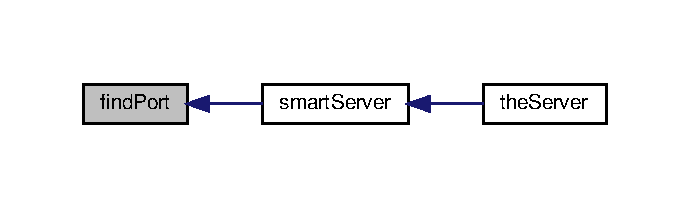
\includegraphics[width=331pt]{server_8h_a2cdb41d0910c3a1d4b82668182dd8a33_icgraph}
\end{center}
\end{figure}
\mbox{\Hypertarget{server_8h_a7751c5c6e765ed5ce531c15904682eab}\label{server_8h_a7751c5c6e765ed5ce531c15904682eab}} 
\index{server.\+h@{server.\+h}!get\+Mime\+Type@{get\+Mime\+Type}}
\index{get\+Mime\+Type@{get\+Mime\+Type}!server.\+h@{server.\+h}}
\subsubsection{\texorpdfstring{get\+Mime\+Type()}{getMimeType()}}
{\footnotesize\ttfamily char$\ast$ get\+Mime\+Type (\begin{DoxyParamCaption}\item[{char $\ast$}]{name }\end{DoxyParamCaption})}



T\+Function name\+: get\+Mime\+Type This function is used to determine the mime-\/type of the file passed in as a paramter. It extracts the file extension of the filename passed in as. 


\begin{DoxyParams}{Parameters}
{\em name} & and searches the mime-\/types.\+tsv file for the appropriate mime-\/type.\\
\hline
\end{DoxyParams}
If the appropriate mime-\/type is found, it is returned as a char$\ast$, if not, the application/octet-\/stream mime-\/type is returned to indicate to the client that the mime-\/type for the file is unknown.

If a user wishes to add a mime-\/type + file extension combination to improve compatiblity, they may do so by editing the mime-\/types.\+tsv file found in the root directory of the server. Ensure that the format is adhered to and the number found on the first line of the file is incremented to ensure that the newly added mime-\/type is considered.


\begin{DoxyParams}{Parameters}
{\em name} & -\/ char$\ast$ pointing to a C-\/\+Style string containing the path to file to be sent to client. \\
\hline
\end{DoxyParams}
\begin{DoxyReturn}{Returns}
char$\ast$ -\/ the mime-\/type to use for the file requested. 
\end{DoxyReturn}


Definition at line 455 of file server.\+c.

Here is the caller graph for this function\+:\nopagebreak
\begin{figure}[H]
\begin{center}
\leavevmode
\includegraphics[width=350pt]{server_8h_a7751c5c6e765ed5ce531c15904682eab_icgraph}
\end{center}
\end{figure}
\mbox{\Hypertarget{server_8h_ada7020aa14056fa9a6c85f8181ca3d09}\label{server_8h_ada7020aa14056fa9a6c85f8181ca3d09}} 
\index{server.\+h@{server.\+h}!parse\+Request@{parse\+Request}}
\index{parse\+Request@{parse\+Request}!server.\+h@{server.\+h}}
\subsubsection{\texorpdfstring{parse\+Request()}{parseRequest()}}
{\footnotesize\ttfamily char$\ast$ parse\+Request (\begin{DoxyParamCaption}\item[{char $\ast$}]{temp }\end{DoxyParamCaption})}



Function name\+: parse\+Request This function processing the request received from the client. Since the ssl server only supports \char`\"{}\+G\+E\+T\char`\"{} http requests, it scans the request received given in. 


\begin{DoxyParams}{Parameters}
{\em temp,for} & the directory of the file requested.\\
\hline
\end{DoxyParams}
The requested file is then returned. If a requested file could not be found in the request header, due to H\+T\+TP protcol version mismatches or any other unknown reason, N\+U\+LL is returned.


\begin{DoxyParams}{Parameters}
{\em temp} & -\/ char$\ast$ poinuting to a C-\/\+String containing the request received from the client. \\
\hline
\end{DoxyParams}
\begin{DoxyReturn}{Returns}
char$\ast$ -\/ the requested file from the request header. N\+U\+LL if a file path could not be found in the request header. 
\end{DoxyReturn}


Definition at line 185 of file server.\+c.

Here is the caller graph for this function\+:\nopagebreak
\begin{figure}[H]
\begin{center}
\leavevmode
\includegraphics[width=350pt]{server_8h_ada7020aa14056fa9a6c85f8181ca3d09_icgraph}
\end{center}
\end{figure}
\mbox{\Hypertarget{server_8h_a02ad7b3294dd3cdda69bb9295aaaf7ed}\label{server_8h_a02ad7b3294dd3cdda69bb9295aaaf7ed}} 
\index{server.\+h@{server.\+h}!send\+File@{send\+File}}
\index{send\+File@{send\+File}!server.\+h@{server.\+h}}
\subsubsection{\texorpdfstring{send\+File()}{sendFile()}}
{\footnotesize\ttfamily void send\+File (\begin{DoxyParamCaption}\item[{B\+IO $\ast$}]{socket,  }\item[{char $\ast$}]{file\+Name,  }\item[{char $\ast$}]{status\+Code }\end{DoxyParamCaption})}



Function name\+: send\+File This function sends or writes the appripate file to the B\+IO object/socket connected to the client. The function attempts to open the file with the path given by. 


\begin{DoxyParams}{Parameters}
{\em file\+Name} & and writes the file in \char`\"{}chunks\char`\"{} of 2048 bytes. The contents of the opened file is read into a buffer and the contents of the buffer are written to the socket until the end of the file has been reached. The file is read at a rate of 2048 bytes per write. Once the entire contents of the file has been written the B\+IO object is flushed to ensure all data is sent and the function returns.\\
\hline
\end{DoxyParams}
This function first constructs the appropriate response header, sends the response header, thereafter sending or writing the requested file.

If the file could not be opened, due to it not existing in the root directory or sub-\/directory of the ssl server program, the function returns without writing anything to the client.


\begin{DoxyParams}{Parameters}
{\em socket} & -\/ B\+I\+O$\ast$ to a B\+IO object connecting the client to the ssl server. \\
\hline
{\em file\+Name} & -\/ char$\ast$ pointing to a C-\/\+String containing the requested file \\
\hline
{\em status\+Code} & -\/ char$\ast$ pointing to a C-\/\+String containing the appropiate status code to send to the client within the response header. \\
\hline
\end{DoxyParams}


Definition at line 328 of file server.\+c.

Here is the call graph for this function\+:\nopagebreak
\begin{figure}[H]
\begin{center}
\leavevmode
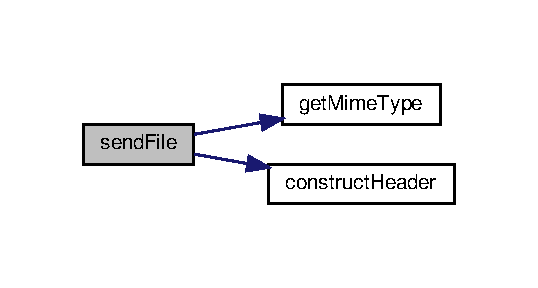
\includegraphics[width=258pt]{server_8h_a02ad7b3294dd3cdda69bb9295aaaf7ed_cgraph}
\end{center}
\end{figure}
Here is the caller graph for this function\+:\nopagebreak
\begin{figure}[H]
\begin{center}
\leavevmode
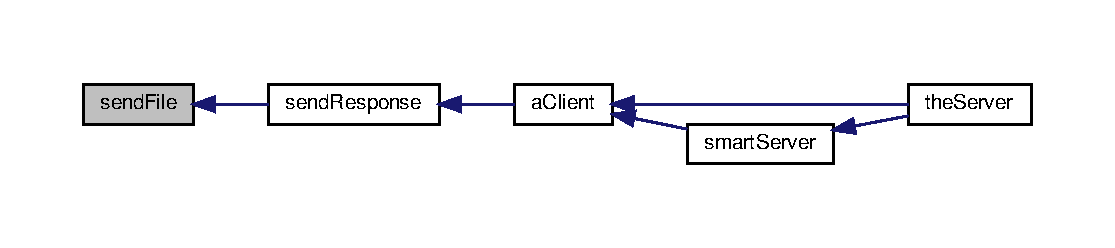
\includegraphics[width=350pt]{server_8h_a02ad7b3294dd3cdda69bb9295aaaf7ed_icgraph}
\end{center}
\end{figure}
\mbox{\Hypertarget{server_8h_a9162818fd6dab1ab1d6ea625b9fd6b12}\label{server_8h_a9162818fd6dab1ab1d6ea625b9fd6b12}} 
\index{server.\+h@{server.\+h}!send\+Response@{send\+Response}}
\index{send\+Response@{send\+Response}!server.\+h@{server.\+h}}
\subsubsection{\texorpdfstring{send\+Response()}{sendResponse()}}
{\footnotesize\ttfamily void send\+Response (\begin{DoxyParamCaption}\item[{B\+IO $\ast$}]{socket,  }\item[{char $\ast$}]{resource }\end{DoxyParamCaption})}



Function name\+: send\+Response This function is used to send the requested file given by. 


\begin{DoxyParams}{Parameters}
{\em resource} & to the client connected on \\
\hline
{\em socket.} & If the resoure is N\+U\+LL signalling that the request header was malformed, the page not found error html page is sent as a response to the client.\\
\hline
\end{DoxyParams}
If the ressource requested points to a directory or the requested file is not found, the page not found error page is sent as a response to the client.

If client sends a G\+ET / request to the server, the default index.\+html homepage is sent as a response.

If the requested resource could be found the server root directrory or sub directroy, it is sent to the client. The main purpose of this function is to determine which response is sent to the clinet. It calls the send\+File function to send/write the appropriate file to the B\+IO socket.


\begin{DoxyParams}{Parameters}
{\em socket} & -\/ B\+I\+O$\ast$ pointing to the B\+IO object on which the client is paired/connected. \\
\hline
{\em resource} & -\/ char$\ast$ pointing to a c-\/string object conting the path to the requested resoure received from the clinet. N\+U\+LL if the client sent a malformed request. \\
\hline
\end{DoxyParams}


Definition at line 228 of file server.\+c.

Here is the call graph for this function\+:\nopagebreak
\begin{figure}[H]
\begin{center}
\leavevmode
\includegraphics[width=350pt]{server_8h_a9162818fd6dab1ab1d6ea625b9fd6b12_cgraph}
\end{center}
\end{figure}
Here is the caller graph for this function\+:\nopagebreak
\begin{figure}[H]
\begin{center}
\leavevmode
\includegraphics[width=350pt]{server_8h_a9162818fd6dab1ab1d6ea625b9fd6b12_icgraph}
\end{center}
\end{figure}
\mbox{\Hypertarget{server_8h_a180f1d916084d821a9e99136064ab071}\label{server_8h_a180f1d916084d821a9e99136064ab071}} 
\index{server.\+h@{server.\+h}!smart\+Server@{smart\+Server}}
\index{smart\+Server@{smart\+Server}!server.\+h@{server.\+h}}
\subsubsection{\texorpdfstring{smart\+Server()}{smartServer()}}
{\footnotesize\ttfamily void$\ast$ smart\+Server (\begin{DoxyParamCaption}{ }\end{DoxyParamCaption})}



Function name\+: smart\+Server. This function is a multithreaded function called when the requested port or default port for the S\+SL server could not be binded to, due to the port being blocked, restricted or already reserved. 

This function attempts to bind to an alternate port within the range 4000-\/4049. If no port within this range could be binded to the function ends the program, alerts; the user that no port could be found and requests the user re-\/run the ssl server with an alternate port speciifed.

If a port could be binded to it functions in the same manner as the function the\+Server. See function\+: the\+Server.

\begin{DoxyReturn}{Returns}
void$\ast$ -\/ N\+U\+LL to signify the end of the thread. 
\end{DoxyReturn}


Definition at line 378 of file server.\+c.

Here is the call graph for this function\+:\nopagebreak
\begin{figure}[H]
\begin{center}
\leavevmode
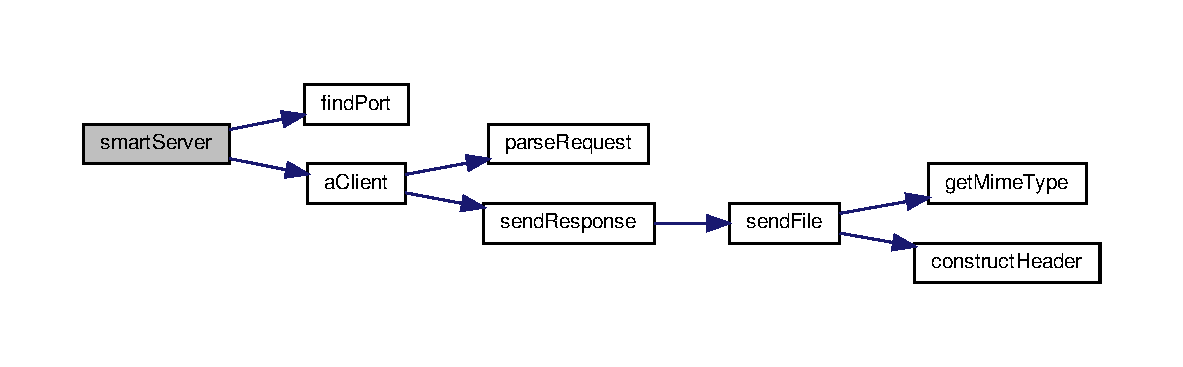
\includegraphics[width=350pt]{server_8h_a180f1d916084d821a9e99136064ab071_cgraph}
\end{center}
\end{figure}
Here is the caller graph for this function\+:\nopagebreak
\begin{figure}[H]
\begin{center}
\leavevmode
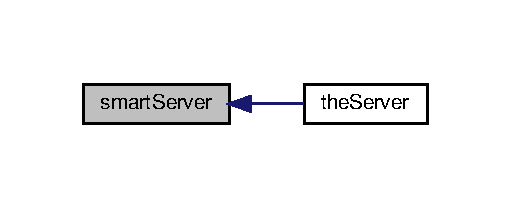
\includegraphics[width=245pt]{server_8h_a180f1d916084d821a9e99136064ab071_icgraph}
\end{center}
\end{figure}
\mbox{\Hypertarget{server_8h_a12f20281e4906f4d25c7c059993ddbc1}\label{server_8h_a12f20281e4906f4d25c7c059993ddbc1}} 
\index{server.\+h@{server.\+h}!the\+Server@{the\+Server}}
\index{the\+Server@{the\+Server}!server.\+h@{server.\+h}}
\subsubsection{\texorpdfstring{the\+Server()}{theServer()}}
{\footnotesize\ttfamily void$\ast$ the\+Server (\begin{DoxyParamCaption}\item[{void $\ast$}]{bio\+Ptr }\end{DoxyParamCaption})}



Function name\+: the\+Server. Intended use is as a multithreaded function. Used to thread the server listening on a port. Should the server not be able to bind the specifed port, it will spawn a new thread to the \hyperlink{server_8h_a180f1d916084d821a9e99136064ab071}{smart\+Server()} function in order to find a reasonable open port and this function will end. Should the server have the ability to bind to the specified port, it will bind to it and run and inifinite loop listening for socket connections on that port. Once a client attempts to make a connection, the function will spawn a new thread for that client -\/ running the \hyperlink{server_8h_af7fd23153c3e547bf7dcde194ffce209}{a\+Client()} function allowing for multiple clients to be handled simultaneously, each within its own thread. 


\begin{DoxyParams}{Parameters}
{\em bio\+Ptr} & -\/ B\+I\+O$\ast$ pointing to a B\+IO object with the ssl and tcp wrapping already implemented to enable a listening socket \\
\hline
\end{DoxyParams}
\begin{DoxyReturn}{Returns}
void$\ast$ -\/ Returns N\+U\+LL, since the intended use is as a P\+O\+S\+IX threaded function 
\end{DoxyReturn}


Definition at line 68 of file server.\+c.

Here is the call graph for this function\+:\nopagebreak
\begin{figure}[H]
\begin{center}
\leavevmode
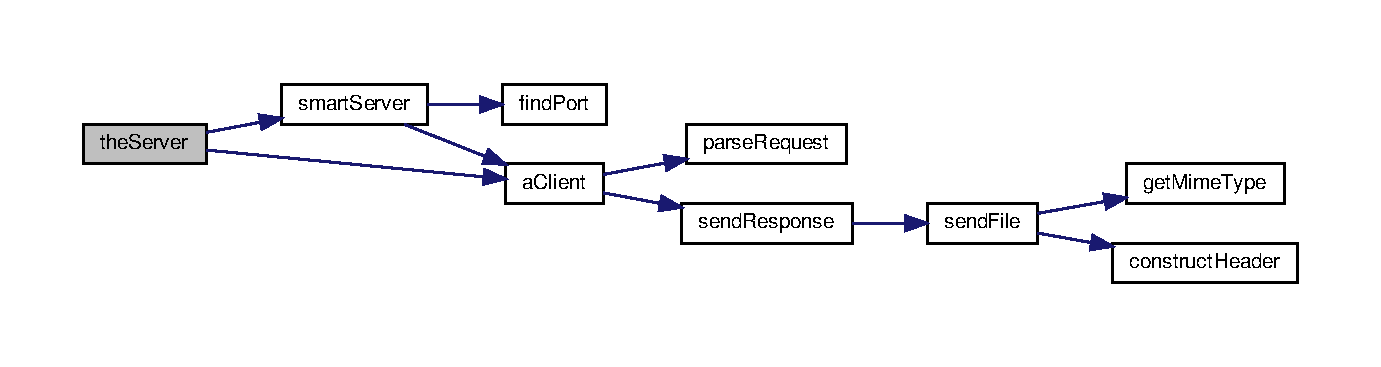
\includegraphics[width=350pt]{server_8h_a12f20281e4906f4d25c7c059993ddbc1_cgraph}
\end{center}
\end{figure}

\input{server_main_8c}
%--- End generated contents ---

% Index
\backmatter
\newpage
\phantomsection
\clearemptydoublepage
\addcontentsline{toc}{chapter}{Index}
\printindex

\end{document}
